\documentclass[12pt]{report} %taille de la police par défaut, et équations jusitifées à gauche
\usepackage[top=3cm,bottom=3cm,left=3.2cm,right=3.2cm,headsep=10pt,a4paper]{geometry}
\usepackage{xcolor}
\definecolor{enstabGreen}{HTML}{C8D200} 	%vert  	#c8d200 
\definecolor{enstabLightGreen}{HTML}{E9ED99} 	%vert  	#c8d200 
\definecolor{enstabLightBlue}{HTML}{009EE0} %bleu clair 	#009ee0
\definecolor{enstabVeryLightBlue}{HTML}{99D8F3} %bleu clair 	#009ee0
\definecolor{enstabDarkBlue}{HTML}{005C8F}	%bleu foncé 	#005c8f
\definecolor{enstabDarkGrey}{HTML}{333333}	%gris fort 	#333333
\definecolor{enstabLightGrey}{RGB}{48,48,48}	%gris fort 	#333333
\definecolor{enstabParme}{HTML}{8878B2}		%parme 	#8878b2
\definecolor{enstabOrange}{HTML}{F18E00} 	%orange 	#f18e00
\usepackage[colorlinks=true,
        urlcolor=enstabLightBlue,
        anchorcolor=enstabDarkBlue,
        linkcolor=enstabDarkBlue,
        citecolor=enstabDarkGrey,
        pdfauthor={O. Reynet},
        pdfkeywords={LaTeX; Report},
        pdftitle={How to produce a report with LaTeX},
        pdfsubject={yours !}] {hyperref}
\usepackage{url}
\usepackage[utf8]{inputenc} % lettres accentuées
\usepackage[T1]{fontenc}    % Use 8-bit encoding that has 256 glyphs
\usepackage[english]{babel} % Pour le français
\usepackage{eso-pic}        % pour une image en fond, page de titre
\usepackage{graphicx}       % Pour inclure des images
\graphicspath{{images/}}    % Où sont les images ?

\usepackage{listings}      % Pour coloriser les codes que vous insérez
\lstset{ %
  backgroundcolor=\color{white},   % choose the background color; you must add \usepackage{color} or 
  basicstyle=\footnotesize\ttfamily,        % the size of the fonts that are used for the code
  breakatwhitespace=false,         % sets if automatic breaks should only happen at whitespace
  breaklines=true,                 % sets automatic line breaking
  captionpos=b,                    % sets the caption-position to bottom
  commentstyle=\color{enstabOrange},    % comment style
  deletekeywords={...},            % if you want to delete keywords from the given language
  escapeinside={\%*}{*)},          % if you want to add LaTeX within your code
  extendedchars=true,              % lets you use non-ASCII characters; for 8-bits encodings only, does not work with UTF-8
  %frame=single,                    % adds a frame around the code
  keepspaces=true,                 % keeps spaces in text, useful for keeping indentation of code (possibly needs columns=flexible)
  keywordstyle=\color{enstabDarkBlue},       % keyword style
  %language=Octave,                 % the language of the code
  morekeywords={*,...},            % if you want to add more keywords to the set
  numbers=left,                    % where to put the line-numbers; possible values are (none, left, right)
  numbersep=8pt,                   % how far the line-numbers are from the code
  numberstyle=\tiny\color{enstabDarkGrey}, % the style that is used for the line-numbers
  rulecolor=\color{black},         % if not set, the frame-color may be changed on line-breaks within not-black text (e.g. comments (green here))
  showspaces=false,                % show spaces everywhere adding particular underscores; it overrides 'showstringspaces'
  showstringspaces=false,          % underline spaces within strings only
  showtabs=false,                  % show tabs within strings adding particular underscores
  stepnumber=5,                    % the step between two line-numbers. If it's 1, each line will be numbered
  stringstyle=\color{enstabParme},     % string literal style
  tabsize=2,                       % sets default tabsize to 2 spaces
  title=\lstname                   % show the filename of files included with \lstinputlisting; also try caption instead of title
}





\usepackage{booktabs}       % pour de jolis tableaux
%\usepackage{fancyhdr}       % pour des entêtes et pieds de pages améliorés.
\usepackage{url}
\usepackage{hyperref}
\usepackage{makeidx}        % requis pour faire les index
\usepackage{amsmath}
\usepackage{amsfonts}
\usepackage{amssymb}
\usepackage{color}
\usepackage{array}
\usepackage{graphicx}
\usepackage{caption} 
\usepackage{hyperref}
\usepackage{algorithm}
\usepackage{algorithmic}
\usepackage{times}
\usepackage{enumitem}
\usepackage{tabularx}     % Ce fichier contient tous les packages nécessaires à la compilation

\begin{document}
\renewcommand{\contentsname}{Contents}	% Nom pour la table des matières
\renewcommand{\bibname}{Bibliography}	% Nom pour les références bibliographiquessss

%----------------------------------------------------------------------------------------
%	PAGE DE GARDE
%----------------------------------------------------------------------------------------

\begingroup
\thispagestyle{empty}
\AddToShipoutPicture*{\put(6,5){
\includegraphics[scale=1]{FondTitreSPID}}} % Image background
\begin{center}
\vspace*{2cm}
{\Huge \textsc{\textbf{System Application Report}}}\\


\vspace*{2cm}
{\huge SWARM SLAM}\par % Intitulé du projet
\end{center}
\begin{figure}[H]
\centering
  %  \includegraphics[trim={1cm 1cm 0.7cm 5cm},clip, scale=0.6]{biscay.png}
\end{figure}

\vspace*{1.5cm}
\textbf{\large by:} 
\begin{center}
{\large
\begin{tabular}{cc}
Elouan Autret \\
\end{tabular}}
\end{center}


\vspace*{1.5 cm}
{\large \textbf{Under the supervision of:}}\\
\begin{center}
{\large
Luc Jaulin\\
Fabrice Le Bars\\}
\end{center}
\endgroup



%----------------------------------------------------------------------------------------
%	SOMMAIRE
%----------------------------------------------------------------------------------------
\tableofcontents  % Imprime le sommaire
\cleardoublepage  % pour commencer sur une page impaire


%----------------------------------------------------------------------------------------
%	Préambules
%----------------------------------------------------------------------------------------
\chapter*{Acknowledgement}
\addcontentsline{toc}{chapter}{Acknowledgement}

First of all, I would like to thank my supervisor during the project,Luc Jaulin, who were available for all my interrogations and ensured that I was not overwhelmed by my pretensions.

I also would like to thanks Simon Rohou and Thomas Le Mézo for supporting my incessant interruptions for information requests on Ibex and discussing my  work.

And finally, I would like to thank Jordan Ninin for his help in improving the efficiency of my program.
%%
%%
\listoffigures  % table des figures
%\listoftables   % table des tableaux
%%%----------------------------------------------------------------------------------------
%%%	PART I 
%%%----------------------------------------------------------------------------------------
\chapter*{Introduction}
\addcontentsline{toc}{chapter}{Introduction}
In recent years the world has seen a multiplication of robots (we will consider a robot as a machine which does not need human interactions during its runtime in the doing of its task – for example an autonomous robot instead of a remotely operated vehicles-) but they stay mainly in known places it is sure for robots that does not need to move but, even for mobile robots such as factory robot that have to move products, they generally do not go in unknown places. This is because a robot needs a good localization to carry out its tasks. In outdoor and open environment this localization can be given by a GPS (Global Positioning System) like for the Google Car, an autonomous vehicle that can go into traffic. But in some environments this information is not available, underwater and in covert environments (indoor, dense forest). In such places the robot has to ask itself two questions:\\

-	What is my environment?\\

-	Where am I?\\

Those questions correspond to the SLAM problem, SLAM is an acronym for Simultaneous Localization and Mapping, this corresponds to the situation of the chicken and the egg because to know where is the robot must know the map and to map the environment it needs to know it.\\

The context of our problem is the localization of underwater vehicles in order to explore the environment (to detect mines for example), their localization would be done with the help of beacons with unknown positions (dropped on the zone before the manoeuvre).  This problem can be considered as a SLAM problem.\\
More than one robot would be deployed, this means that they can collaborate in order to be more efficient, for faster exploration and more adaptable. Using multiple robots can be viewed as using a swarm of robots, and  for the swarm to be efficient, it can be useful for the robots to share the information and their mapping data (this can be used to avoid robots exploring the same area)  this initiates the problem of the map merging.\\

This report will explain different methods of SLAM and map merging with the goal of choosing one that will be more appropriate for the task.Then it will present the chosen method and its implementation.

%%
\chapter{Status Report}
\section{Representation}
In general a slam output will give either a topological map or an Occupancy Grid\\

\subsection{Topological Map}

If the algorithm for the SLAM uses landmarks there is chance that it uses a topological map. This type of map will put in relation different landmarks as a graph, the nodes will be the landmarks and the arc can be the path, the distance between the landmarks, for example an underground map is a topological map with stations such as the landmarks and relations are the connections between the stations:\\

\begin{figure}[H]
\centering
    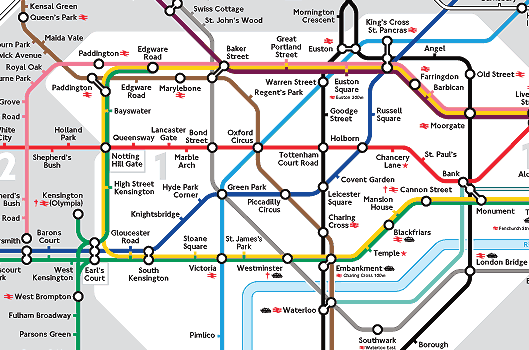
\includegraphics[scale=0.3]{topo.png} 
    \caption{Example of a topological map.}
    \label{fig:topoExample}
\end{figure}

This type of map will be made when sensors can distinguish features in the environment. This type of map has a higher abstraction level, it does not know the metrics of the environment but it can consider objects in it:

\begin{figure}[H]
\centering
    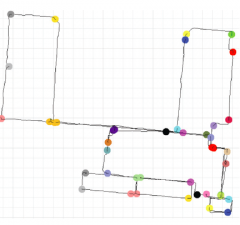
\includegraphics[scale=0.6]{topo2.png} 
    \caption{Example of a SLAM topological map \cite{Ranganathan10ijrr}.}
    \label{fig:topo2Example}
\end{figure}

 In figure~\ref{fig:topo2Example} the landmarks are corners and intersections. 

\subsection{Occupancy Grid}

An occupancy grid will represent the continuous space divided in a 2 or 3D grid where each square or box contains the probability of being occupied, in figure 3 the squares are in a trinary state (empty , occupied or unknown):


\begin{figure}[H]
\centering
    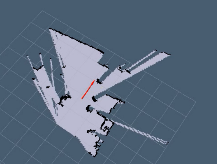
\includegraphics[scale=2.2]{occupGrid.png} 
    \caption{2D Occupancy Grid of the Robotic Club in ENSTA Bretagne with Hector Slam~\cite{kohlbrecher2011flexible}.}
    \label{fig:occupGrid}
\end{figure}
\section{Classical methods for SLAM}
In general when using a SLAM the state equation of the robot is known and helps the localization problem, the state equation models the behaviour of the robot in function of input parameters:

\begin{align}
\dot{x} &= v*cos(\theta)\\
\dot{y} &= v*sin(\theta)\\
\dot{\theta} &= u_{1}\\
\dot{v} &= u_{2}
\end{align}

Above is a state equation modelling a car ($x$ and $y$ are the position, $\theta$ is the heading and v the speed), with input $u_{1}$ and $u_{2}$ which are known (the robot computes them).
They are the most used and studied method and many use probability and decision theory to estimate the pose of the robots and the map such as the EKF Slam.

\subsection{EKF SLAM}
An EKF SLAM is a slam algorithm that uses the Extended Kalman filter to accomplish the problem, it is a features based slam.

\subsubsection{Kalman Filter}

The Kalman Filter is used to estimate the linear state equation variable over time keeping track of the uncertainties of the variables, this filter permits data fusion:

\begin{figure}[H]
\centering
    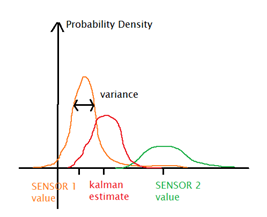
\includegraphics[scale=1]{kalmanExample.png} 
    \caption{Simple example of data fusion.}
    \label{fig:kalexample}
\end{figure}

If we have two sensors that measure the same variable the Kalman filter will combine them in function of their variances (a sensor with great variance means that it is less precise so it is less trustworthy whereas a sensor with little variance will be more precise), in figure~\ref{fig:kalexample} we combine two sensors with a Gaussian noise, this is a simple example of what the Kalman filter can do, it can also combine information between the state variables, (a state variable can be the position, the speed, angular speed ) and if we have relations between those variables (position and speed) the Kalman filter will be able to combine the estimates.\\

Therefore in what way is the Kalman filter used for the slam? The landmarks detected are put in the state equation in order to estimate their position and use them to improve the robot localisation:

\begin{figure}[H]
\centering
    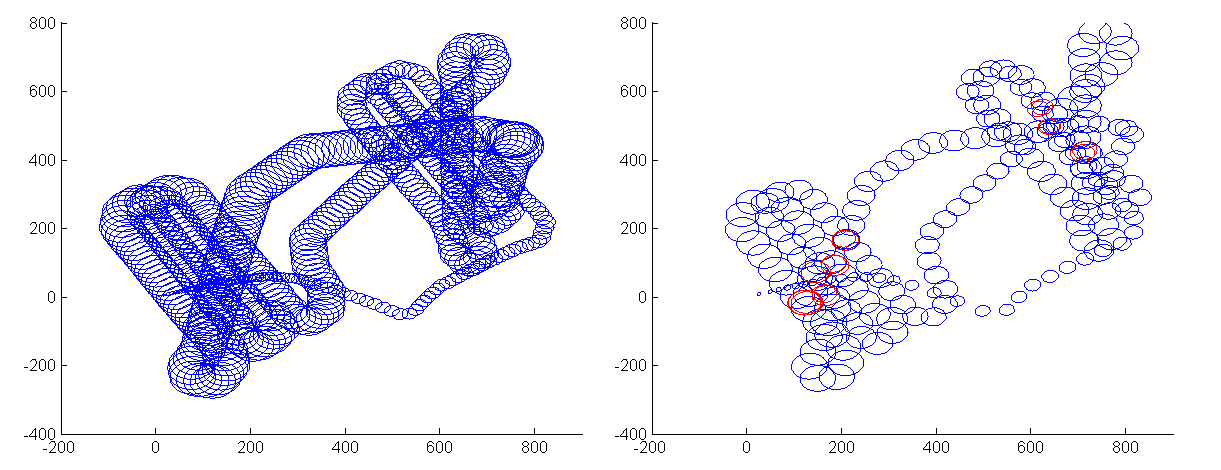
\includegraphics[scale=0.5]{observerKalman.png} 
    \caption{Estimate of position of an underwater vehicle without and with landmarks using a Kalman Filter.}
    \label{fig:obserKalman}
\end{figure}

In figure~\ref{fig:obserKalman} the Kalman filter only uses the model of the underwater vehicle to estimate its position therefore the variance (represented by an ellipse) always increases whereas when landmarks are available it can slow the uncertainty propagation. The extended Kalman filter is used to work on nonlinear problems such as the SLAM problem, thus causing a bit of approximation.

\subsection{FastSLAM}

The FastSLAM algorithm \cite{montemerlo2002fastslam} uses a particle filter and a Kalman filter to solve the SLAM problem, so this is also a landmark based algorithm.\\
The FastSLAM algorithm creates many particles that represent hypothesis on the position of the robot, the particles are randomly placed over the possible position of the robot. Then the landmarks are estimated for each particle using the Extended Kalman filter (supposing the position of the robot known for the particle).\\

After that the likeliness of each particle being the right hypothesis is computed. Some particles will be more likely to be right than others, therefore a resampling is done near the most likely particles found just before, the particles are now with the same likeliness (weight). The particles are kept through time and are updated (with each particle having different movements and new weights depending of the movement likeliness). Through time, the particles are supposed to regroup around the correct position of the robot \cite{sven13}.
\section{SLAM via Interval Analysis}
\label{sec:slamIA}
The methods seen approach the problem from a probabilistic point of view but, are not guaranteed, it relies on the probability of the robot to not be an outlier, and when we need a sure position of the robot it could lead to a failure (in a harmful environment or in interaction with humans it would be hazardous). The interval analysis means to guarantee the result, and is not subject to approximation because it does not need to linearise the problem. Interval Analysis has grown to be a competent alternative to the probabilistic methods.

\subsection{Interval Analysis}
\label{sec:srIA}
In the Intervals theory a real number is replaced by an interval with an uncertainty represented by its width that includes the right number, for a known x the corresponding interval could be $[ \,x,-\epsilon,x+\epsilon] \,$ with a width of $2\epsilon$.

\begin{figure}[H]
\centering
    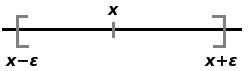
\includegraphics[scale=0.6]{Interval.png} 
    \caption{Representation of an interval.}
    \label{fig:interExample}
\end{figure}

This representation has advantages, to easily manage uncertainties by enclosing them in an interval, but the intervals can be contracted around the feasible value thus reducing the uncertainty.\\

This representation have advantages, to easily manage uncertainties by enclosing them in an interval, but the intervals can be contracted around the feasible value thus reducing the uncertainty.\\
For example considering the sets $X=[\,1,7]\,$ and $Y=[\,-1,5]\,$ and if $Y$ and $X$ are constraint by the equation $y=x^{2}$ then we can contract the set $Y$:\\

$Y = Y\cap X^{2} =[\,1,5]\,$\\

But X can also be contracted by going backwards:\\

$X=X\cap \sqrt{Y} =[\,0,\sqrt{5}]\,$\\

This operation is a forward-backward contractor~\cite{jaulin2001applied} and~\cite{chabert2009contractor}.

\begin{figure}[H]
\centering
    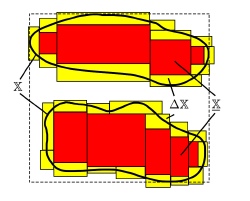
\includegraphics[scale=0.6]{subpaving.png} 
    \caption{Sub paving of a 2 dimensional set \cite{Bet14}.}
    \label{fig:subExample}
\end{figure}


The set inversion \cite{jaulin1993set}, finding $X$ such as $f([\,X]\,)$ is in S, is easy to compute with intervals' arithmetic if X is the solution set (see above, the red boxes are included in the set, yellow boxes are on the border), the minimal size of the boxes correspond to the precision for the set inversion.\\ 
One of the first papers to address the SLAM problem via interval analysis was in \cite{di2004set}, in this paper they proposed an algorithm for the mapping and localization using landmarks.

\begin{figure}[H]
\centering
    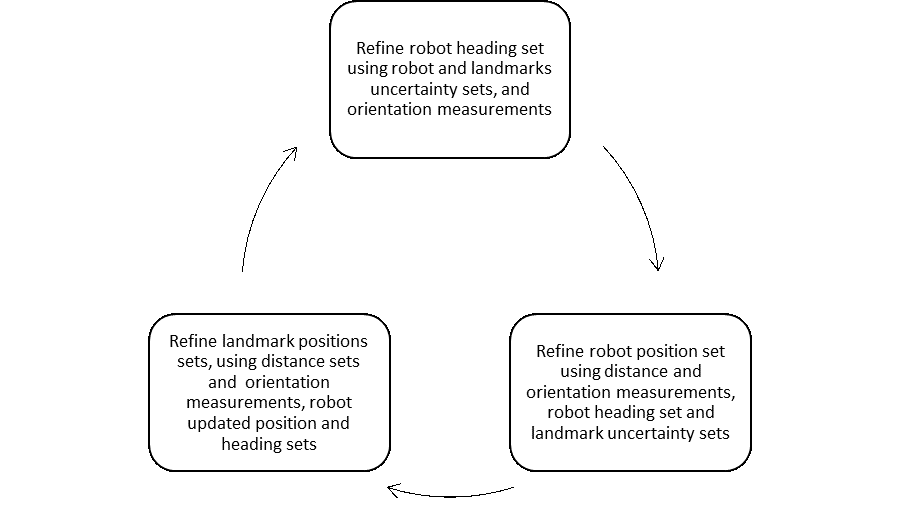
\includegraphics[scale=0.7]{algoslam.png} 
    \caption{Algorithm process for the SLAM \cite{di2004set}.}
    \label{fig:algoslamExample}
\end{figure}

In their case, figure 7, they considered receiving bearing and distance of landmarks, by using constraints propagation (contractors) we can refine the sets \cite{jaulin2010resolution}

\begin{figure}[H]
\centering
    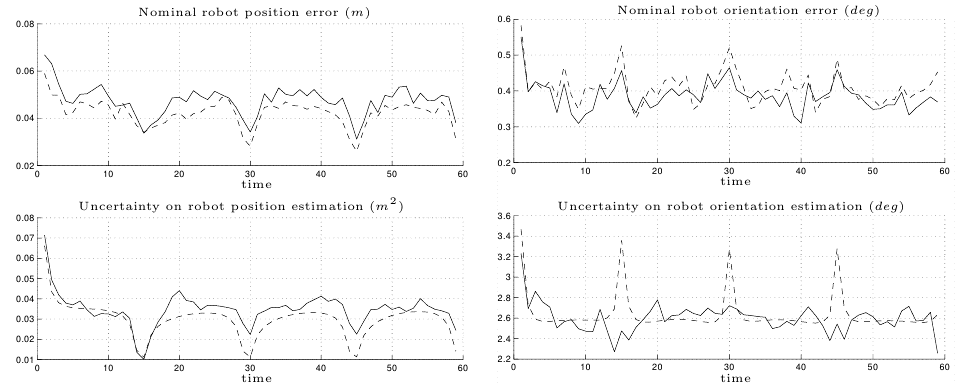
\includegraphics[scale=0.9]{difalgo.png} 
    \caption{Error differences between EKF-SLAM and Interval SLAM in \cite{di2004set}.}
    \label{fig:difalgo}
\end{figure}

The interval method can be as precise as the EKF-SLAM but with having a guaranteed uncertainty.
\section{With Multiple Robots}
By using multiple robots the possibilities are expanded but under certain conditions, such as, they do not interfere with each other and do not redo the work of others. For exploration it means that they have to know where the others are or have been, in order to do that the robots need to merge their map to identify their common or uncommon environments.\\
This problem can be represented as a graph where the nodes are the positions of the robots at a certain time and the arcs are the transformation matrix from a node to another:

\begin{figure}[H]
\centering
    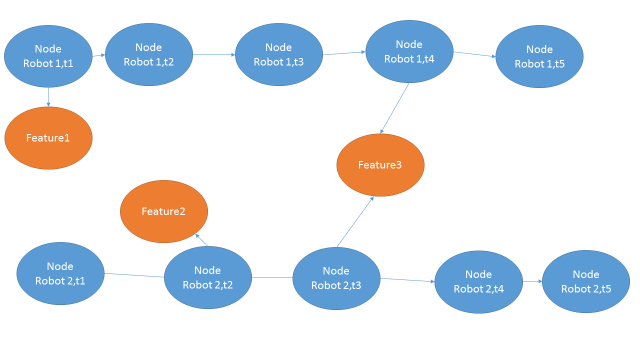
\includegraphics[scale=0.6]{graphslam.png} 
    \caption{Graph representation of the Multi-robot SLAM problem.}
    \label{fig:difalgo}
\end{figure}

The goal of this problem is to make the link between robot 1 and robot 2 (with the feature 3 in figure 9) of course in some contexts a sole link between the graphs would not be sufficient (with sensors getting only range), and would need two or three links two associate the graph.
Another method would be to iterate over each feature from the graph of a robot and try to match it to the features of another graph, it is the same reasoning as the ICP (Iterative Closest Point) method use for matching frames for a 3D mapping.

\section{Direction}
This report allows to conclude that for our project the interval methods is more appropriate (here robots could go near mines so we need a guaranteed localization).The next thing to do is to put our problem into an equation, the SLAM with one robot will be more or less easy as it has been done a few times before, but the map merging has been less studied.

\chapter{Theoretic}
If the context of the mission is established, the property of the robots are not :
  
\begin{itemize}[label=$-$,itemsep=0cm,topsep=0cm]
\item The robots will have a maximum range of intercommunication;
\item The robots will have a maximum range of beacons detection;
\item The robots have access to their heading and speed;
\item The beacons are recognizable;
\item The beacons do not move during the mission;
\item The beacons can ping themselves and transmit the information to the robots;
\item The distance information and communication are not available continuously.
\end{itemize}

\section{SLAM}

As seen in~\ref{sec:slamIA} the SLAM with recognizable landmarks can be done (and has been done) with constraint propagation.

\subsection{One robot}

\subsubsection*{Contractors}\label{sssec:contract}
For the SLAM two contractors are needed (see ~\ref{sec:srIA}), a distance contractor between the robot and a beacon position, for the beacons between themselves (as they can know their distances), a robot state contractor to spread the constraint over the time.

\subparagraph{Distance Contractor}
The Distance contractor is based on a simple function, the euclidean distance:

\begin{equation}
(R_{x}-B_{x})^{2}+(R_{y}-B_{y})^{2} = d_{RB} 
\end{equation}

Where R is the box containing the robot and B the box for the beacon and $d_{RB}$ the interval of the measure. This contractor with the euclidean distance is not very efficient, indeed if the pose of the robot is known but the beacon has not been estimated yet, the output will be the box containing the circle with the measured distance as a rayon surrounding the robot.To improve the computation the contracted box can be cut into a grid and then the different cases would be fed to the contractor and the remaining non-empty boxes would be kept.


\begin{figure}[H]
\centering
    \begin{minipage}[b]{0.4\textwidth}
    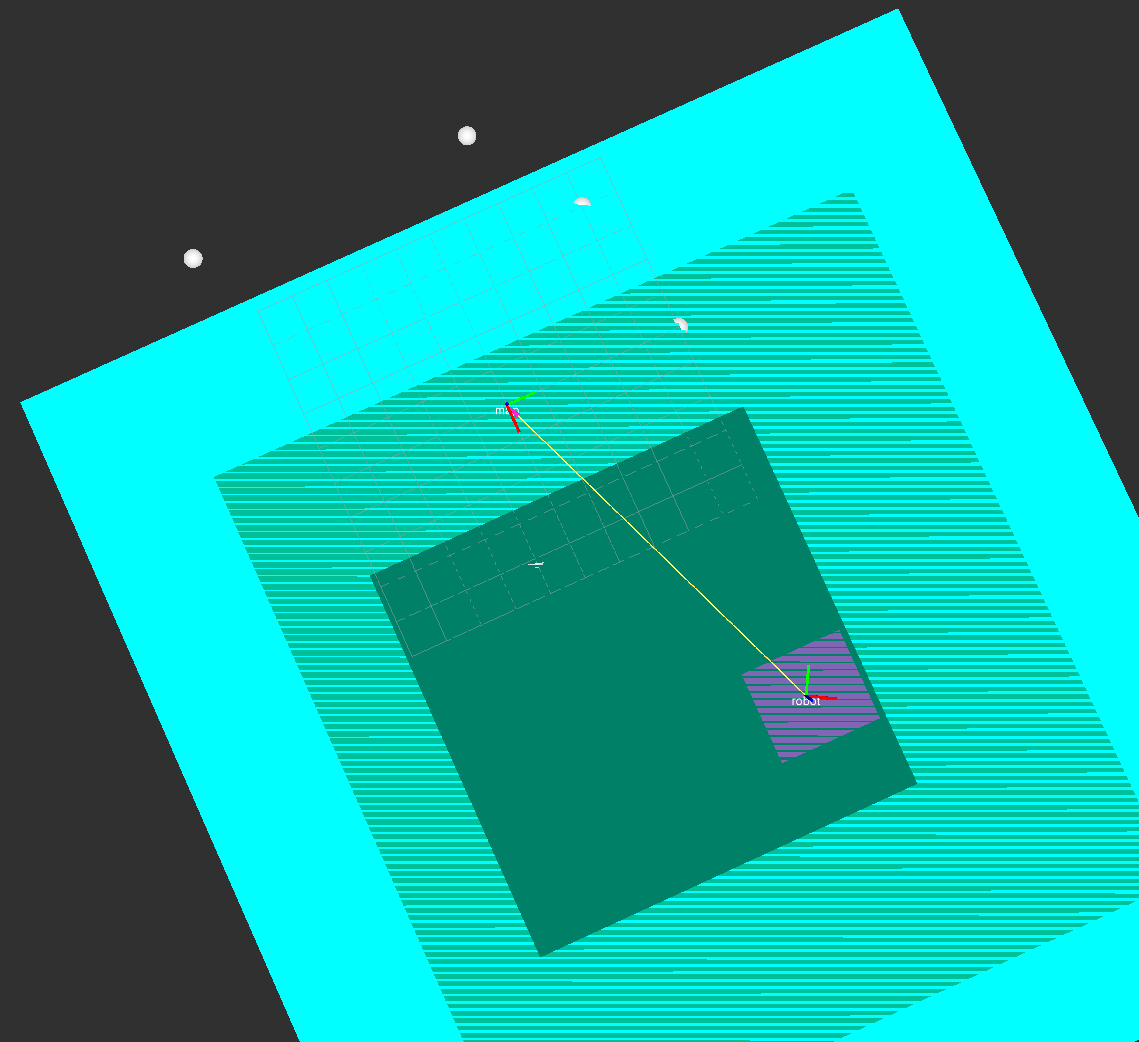
\includegraphics[scale=0.13,angle=0]{picture_no_sivia.png}
    \caption{Beacons Boxes computed without paving.}
    \label{fig:picture_no_sivia}
    \end{minipage}
    \begin{minipage}[b]{0.4\textwidth}
    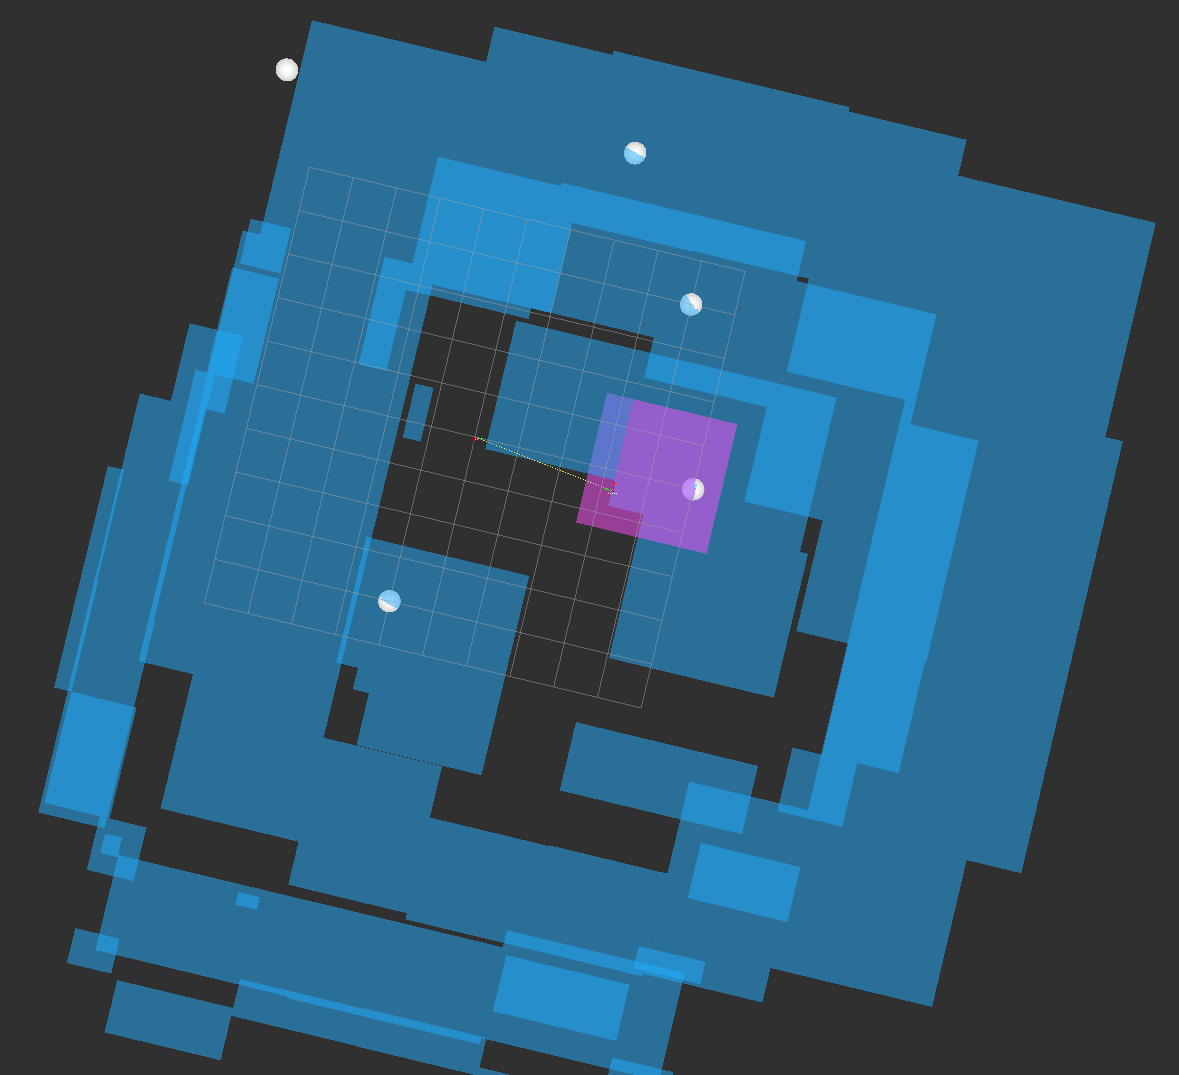
\includegraphics[scale=0.13,angle=0]{sivia_distcontraint.png}
    \caption{Beacons Box computed with paving with SIVIA \cite{jaulin1993set}.}
    \label{fig:sivia_distcontraint}
    \end{minipage}
\end{figure}

In figure~\ref{fig:picture_no_sivia} the position will be difficult to improve and in ~\ref{fig:sivia_distcontraint} the estimates of the beacons are better as the space between the robot and a beacon is not considered as a feasible position.

\subparagraph{Robot State Contractor}

 The interest of this contractor is to use a the contraction made by a beacon a a time $t_{1}$ to improve the estimate the robot over the time which can then improve the estimate of a beacon via a measure at a time $t_{2}$.

The contractor is made by knowing how the robot can move therefore the state equation of the robot is needed, for the report the state equation of a car is used:

\begin{align}
\dot{x} &= v*cos(\theta)\\
\dot{y} &= v*sin(\theta)\\
\dot{\theta} &= u_{1}\\
\dot{v} &= u_{2}
\end{align}

Then considering $u$ the input of the robot, $dt$ the incrementation duration, the time $t_{1}$ and the time $t_{2}=t_{1}+dt$ and $X(t)$ the state vector at the time $t$ the contractor is based on the following equation:  

\begin{align}
X_{0}(t_{2}) &= X_{0}(t_{1}) + X_{3}(t_{1})*\textnormal{cos}(X_{2}(t_{1}))*dt\,\\
X_{1}(t_{2}) &= X_{1}(t_{1}) + X_{3}(t_{1})*\textnormal{sin}(X_{2}(t_{1}))*dt\\
X_{2}(t_{2}) &= X_{2}(t_{1}) + u_{1}*dt\\
X_{3}(t_{2}) &= X_{3}(t_{1}) + u_{2}*dt
\end{align}

\subsubsection*{Combining the information}

The slam is supposed to be online (done in real time) this mean as for the control of a robot an estimate of
the position is needed continuously ( > 10 Hz). At each iteration the algorithm~\ref{alg:iterSlam} is processed.

\begin{algorithm}[H]
\caption{Process information for an iteration }
\label{alg:iterSlam}
\begin{algorithmic}[1]
\REQUIRE $v(t)$,$\theta(t)$,$u(t)$\\
   $X$ : (State vector from the precedent iteration)\\
   $[\,dt]\,$ :(interval containing the duration from the last iteration)\\
   $measure_{beacons}$: (set of measures between two iteration)\\
   $Past$ (vector recording of robot estimate and measure)\\
   $n$(size of Past)\\
   $distC$ : contractor of distance\\
   $robotStateC$ : contractor of robot estimate\\
   $update$: function which update the estimate of X by taking into account the proprioceptive data.\\
   $box_{beacons}$ : Set of the estimate of the beacons  
\STATE $X \leftarrow update(X,[\,dt]\,v(t),\theta(t),u(t)) $
\STATE $Past  \leftarrow Past + \{(X,[\,dt]\,,measure_{beacons})\} $
\STATE $n  \leftarrow n+1 $
\IF{$measure_{beacons} \neq  \emptyset $}
\FOR{$i=n-1;i>1;i--$}
\STATE $(X_{i},[\,dt]\,_{i},measure_{beacons,i}) \leftarrow Past(i)$
\STATE $(X_{i+1},[\,dt]\,_{i+1},measure_{beacons,i+1}) \leftarrow Past(i+1)$
\FOR{$measure_{beacon,i} \in measure_{beacons,i}$}\label{op:distB_1}
\STATE $(X_{i},box_{beacon},measure_{beacon,i}) \leftarrow distC(X_{i},box_{beacon},measure_{beacon,i})$
\ENDFOR
\STATE $(X_{i},X_{i+1},[\,dt]\,_{i+1}) \leftarrow robotStateC(X_{i},X_{i+1},[\,dt]\,_{i+1})$
\ENDFOR
\FOR{$i=0;i<n-1;i++$}
\STATE $(X_{i},[\,dt]\,_{i},measure_{beacons,i}) \leftarrow Past(i)$
\STATE $(X_{i+1},[\,dt]\,_{i+1},measure_{beacons,i+1}) \leftarrow Past(i+1)$
\FOR{$measure_{beacon,i} \in measure_{beacons,i}$}\label{op:distB_2}
\STATE $(X_{i},measure_{beacon,i}) \leftarrow distC(X_{i},measure_{beacon,i})$
\ENDFOR
\STATE $(X_{i},X_{i+1},[\,dt]\,_{i+1}) \leftarrow robotStateC(X_{i},X_{i+1},[\,dt]\,_{i+1})$
\ENDFOR
\ENDIF
\end{algorithmic}
\end{algorithm}

This algorithm does not use all the information available when using one robots (distance between beacons) and does not use a paving for the estimation of the beacons:

When receiving data from a beacon a contractor over the distance between beacon can be computed :

\begin{algorithm}[H]
\caption{Process distance between beacons }
\label{alg:distBetBeaconsSlam}
\begin{algorithmic}[1]
\REQUIRE $measure_{beacons}$: (set of measures between two iteration)\\
   $box_{beacons}$ : Set of the estimate of the beacons\\
   $Bsender$ : beacon which has transmitted the data   
\FOR{$measure_{beacon} \in measure_{beacons}$}\label{op:distB_3}
\STATE $(box_{Bsender},box_{beacon},measure_{beacon}) \leftarrow distC(box_{Bsender},box_{beacon},measure_{beacon})$
\ENDFOR
\end{algorithmic}
\end{algorithm}

But as written in ~\ref{sssec:contract} the estimate box for the beacons can be paved, that change the precedents 
algorithms when treating with a beacon estimate (\ref{op:distB_1},\ref{op:distB_2},\ref{op:distB_3}). A algorithm for the distance constraint between two set of boxes must be done:

\begin{algorithm}[H]
\caption{Distance Constraint Application on two set of boxes }
\label{alg:distTwoSet}
\begin{algorithmic}[1]
\REQUIRE $d$: interval of the distance\\
   $\mathbb{B_{\textnormal{1}}}$ : A set of boxes\\
   $\mathbb{B_{\textnormal{2}}}$ : A second set of boxes
\STATE $\mathbb{T_{\textnormal{1}}} \leftarrow$ Vector of empty boxes of the same size of $\mathbb{B_{\textnormal{1}}}$
\STATE $\mathbb{T_{\textnormal{2}}} \leftarrow$ Vector of empty boxes of the same size of $\mathbb{B_{\textnormal{2}}}$
\FOR{$box_1 \in \mathbb{B_{\textnormal{1}}}$}
\FOR{$box_2 \in \mathbb{B_{\textnormal{2}}}$}
\STATE $(box_{1t},box_{2t},d) \leftarrow distC(box_1,box_2,d)$
\STATE $\mathbb{T_{\textnormal{1}}}(box_1) \leftarrow \mathbb{T_{\textnormal{1}}}(box_1)  \cup box_{1t}$
\STATE $\mathbb{T_{\textnormal{2}}}(box_1) \leftarrow \mathbb{T_{\textnormal{2}}}(box_2)  \cup box_{2t}$
\ENDFOR
\ENDFOR
\STATE $\mathbb{B_{\textnormal{1}}} \leftarrow \mathbb{T_{\textnormal{1}}}\setminus\{box \in \mathbb{T_{\textnormal{1}}} \mid box = \emptyset \}$
\STATE $\mathbb{B_{\textnormal{2}}} \leftarrow \mathbb{T_{\textnormal{2}}}\setminus\{box \in \mathbb{T_{\textnormal{2}}} \mid box = \emptyset \}$
\end{algorithmic}
\end{algorithm}

With the algorithms~\ref{alg:iterSlam},~\ref{alg:distBetBeaconsSlam},~\ref{alg:distTwoSet} it is possible to do a range only slam with a unique robot (see chapter~\ref{ch:results} for more details).

\subsection{With more robots}

When using multiple robots, each robot can obtain the estimations of the map from the other robots (if there is transmission), in the context of the mission the first position is known (the box for the pose estimate has a little width depending on the GPS data) therefore the position of the boxes is sure between the robots. When receiving data from another robots, 

\section{Controlling the robots}
\chapter{Implementation}
\section{ROS}
ROS (Robotic Operating System) is an open source framework made toward robotic application.
The goal of ROS is to propose means to facilitate communication between processes,managing possibilities and make available working algorithms for everyone~\cite{quigley2009ros}.

This framework will be use in this project for communication and visualisation.

\subsection{How it works}

ROS is functioning with nodes, a master and slaves,the master is a ROS process and nodes can be programmed by anyone:

\begin{itemize}[label=$-$,itemsep=0cm,topsep=0cm]
\item The framework is available on many OS (operating system)such as Linux (CPU architecture: ARM x86 x64), Android , Windows, OSX;
\item The programming of the nodes can be done in multiple language : C++, Python, Java, Lua, Lisp, C\#, Go, R, Ruby (from the most supported to the least)
\item Nodes written in different languages can function together.
\end{itemize}

The communication with ROS works with topics,subscriber, and publisher, a publishing node will announce to the master that it is publishing over a topic and the subscribing node will say to the master that it want to listen to a topic. Then if the publisher and the subscriber are on the same topic, the master will transfer data in order for the two other node to communicate directly via TCP/IP or UDP (see figure~\ref{fig:rosTopic}).

\begin{figure}[H]
\centering
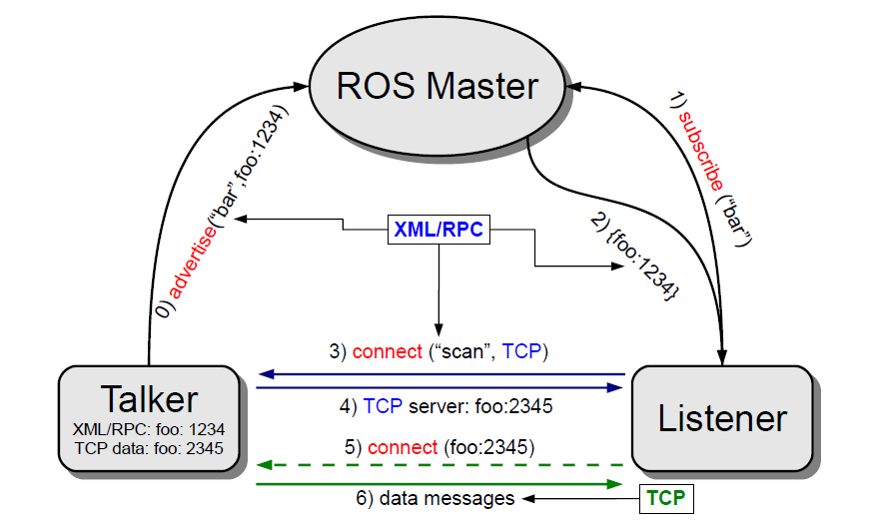
\includegraphics[scale=0.75]{ros_func.png}
\caption{Connection of nodes and topics \cite{rusu13ros}.}
\label{fig:rosTopic}
\end{figure}

ROS also facilitate the serialization of messages (conversion of the message into bytes):\\

\begin{minipage}[b]{0.8\textwidth}
\begin{itemize}[label={},itemsep=0cm,topsep=0cm]
\item std\_msgs/Header header
  \begin{itemize}[label={},itemsep=0cm,topsep=0cm]
  \item uint32 seq
  \item time stamp
  \item string frame\_id
   \end{itemize}
\item geometry\_msgs/Quaternion orientation
  \begin{itemize}[label={},itemsep=0cm,topsep=0cm]
  \item float64 x
  \item float64 y
  \item float64 z
  \item float64 w
  \end{itemize}
\end{itemize}
\end{minipage}


As it can be seen in the message example, a message can reference another message, in order to create message capable of transmitting complex data (an image with all its meta data).
This functionality of ROS permits a big modularity for the programmer, an easy passage from simulation to real via only changing topic names.

\subsection{ROS in the project}

For the simulation of the swarm slam project multiple nodes have been 
created in order to represent accurate communication and sensing.

\subsubsection*{IA\_MSGS}

ia\_msgs is an utility package to regroup created message in order to help to the communication of interval vector (in 2 and 3 dimension):\\

ia\_msgs/StampedInterval
\begin{itemize}[label={},itemsep=0cm,topsep=0cm]
\item std\_msgs/Header header
  \begin{itemize}[label={},itemsep=0cm,topsep=0cm]
  \item uint32 seq
  \item time stamp
  \item string frame\_id
  \end{itemize}
\item ia\_msgs/IdInterval[] data
  \begin{itemize}[label={},itemsep=0cm,topsep=0cm]
  \item uint8 id
  \item ia\_msgs/Interv[] data
    \begin{itemize}[label={},itemsep=0cm,topsep=0cm]
    \item geometry\_msgs/Point position
      \begin{itemize}[label={},itemsep=0cm,topsep=0cm]
      \item float64 x
      \item float64 y
      \item float64 z
      \end{itemize}
    \item float64 width
    \item float64 height
    \end{itemize}
  \end{itemize}
\end{itemize}

The above message allows to send with a time stamp and a reference frame a list of a identified list of two dimensional boxes, used for example to send the estimates of the beacons.

\subsubsection*{RVIZ\_IA\_PLUGIN}

The rviz plug-in has been done to facilitate the visualization of the interval, rviz is on openGL based graphic visualizer incorporated in ROS. rviz can receive message and interpret them.

\begin{figure}[H]
\centering
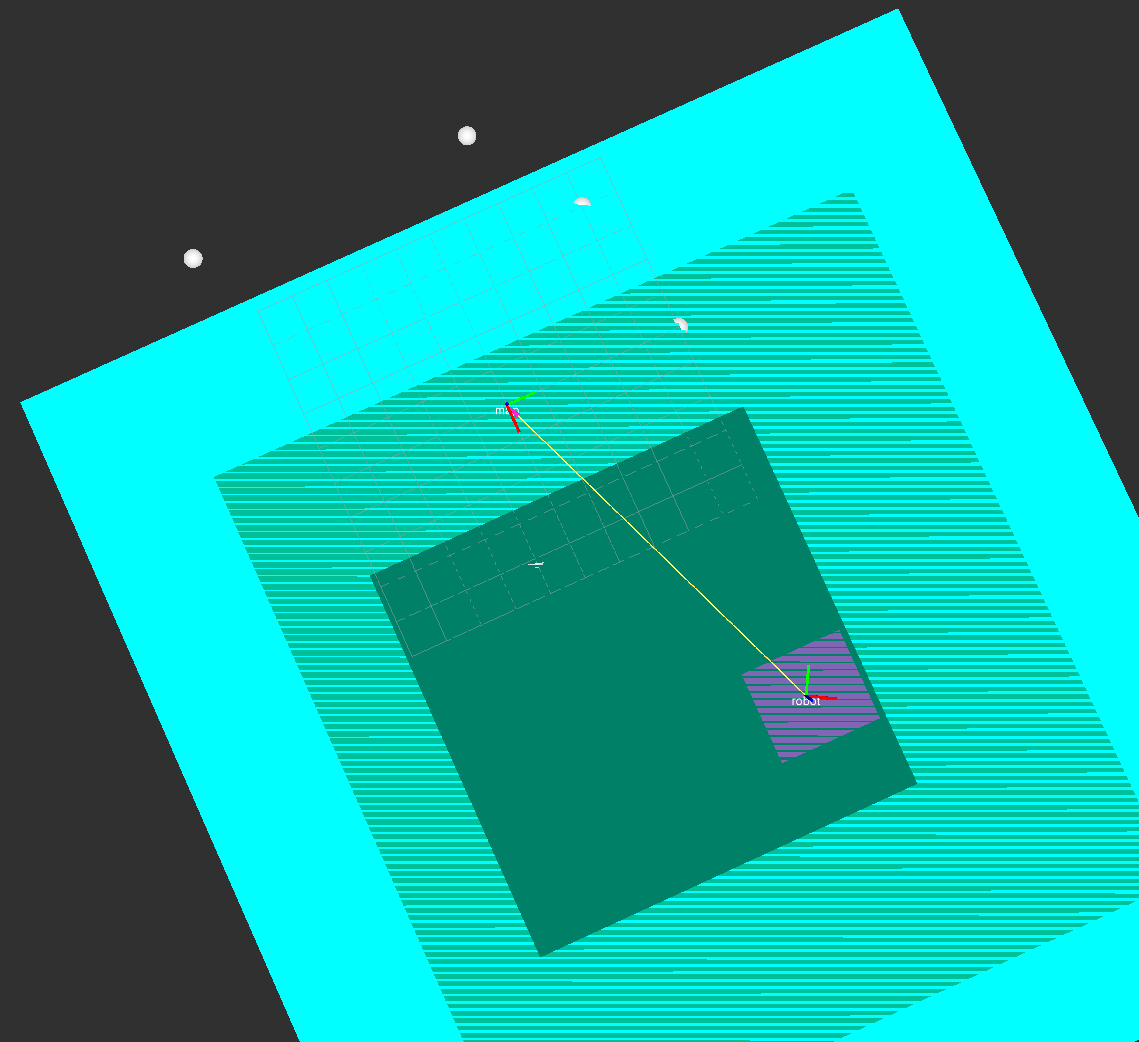
\includegraphics[scale=0.13,angle=0]{picture_no_sivia.png}
\caption{Example of rviz utilisation.}
\label{fig:rvizEx}
\end{figure}

In figure~\ref{fig:rvizEx} rviz interpret the StampedInterval message (the blue rectangle), two frame, the real pose of the robot and the map frame seen as an ensemble of blue green and red arrow, the point cloud of beacons printed as spheres and the Interval message for the pose estimate of the robot.
What has been done is the interpretation of the interval related messages.

\subsubsection*{IA\_SLAM}

It is the core of the project this node receive the sensor data (distance from the beacons), the information from other robots and the proprioceptive data such as the heading,speed motors order, then it estimate the position of the robot and the beacons by using the algorithm from the section~\ref{sec:slamtheory}.It has been implemented in c++ as it create an heavy load on the CPU.

The arithmetic of intervals is done with the help of the IBEX library a c++ library towards intervals applications~\cite{ibex}
\subsubsection*{ROBOT\_SIMU}

This node simulate the robot by using the state equation (a car model for the project) its send the pose information to the beacon\_simu node and the proprioceptive information to the ia\_slam node.This node and all the other simulation nodes have been implemented in Python for easier manipulation.

\subsubsection*{BEACON\_SIMU}

This node simulate the sensor of the beacons,it knows the real pose of the beacons and the pose of the robot and considering the distance from the beacons it send or not the information every second (ia\_slam received a beacon data every tenth of a second).

\subsubsection*{TALK\_SIMU}

This node work on the same principle as the beacon\_simu node but for the discussion between robots, if the robots are close enough data is transferred with a limitation in time,a transfer can only happened three second after another to model the bandwidth limitation with underwater modem, the time was chosen arbitrarily but can be quickly changed.

\subsubsection*{IA\_CONTROLLER}

This node is receiving the position of the robot and the other robots in order to compute the motors orders to follow the path and avoid obstacles. The orders are then send to the robot\_simu node.

\begin{figure}[H]
\centering
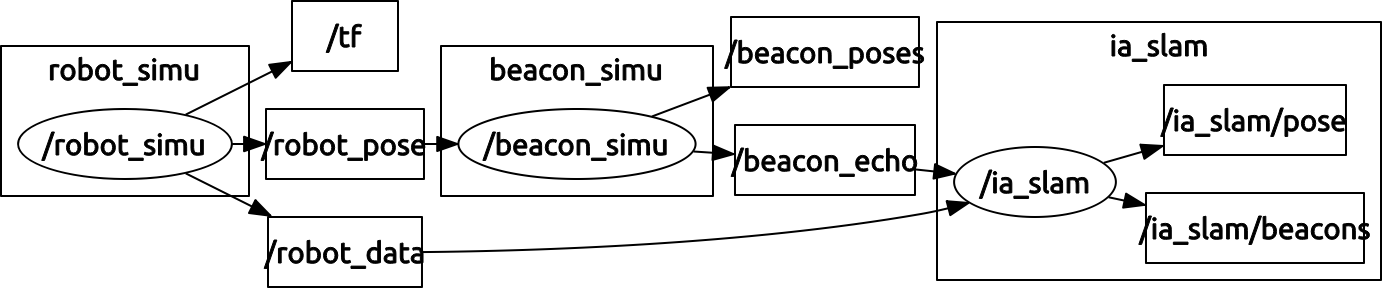
\includegraphics[scale=0.3,angle=0]{simple_slam_ros.png}
\caption{Relation between nodes with one robot and no controller node.}
\label{fig:oneRobGraph}
\end{figure}

In figure~\ref{fig:oneRobGraph} is represented the relation between nodeswith only one robots with the help of rqt\_graph, a ROS program. A  similar graph can be found in the appendix (figure~\ref{fig:completeNode}).
\section{Computational problems}
\subsection{SLAM Heavy Load}

The complexity of the algorithm~\ref{alg:iterSlam} for an iteration is $\sim\mathcal{O}(n.(nbDiv))$ where $n$ is the number of iteration effectuated and $nbDiv$ the maximum number of division of the estimate of the beacons.

Therefore a such an algorithm is not viable for an online slam. The use of the precedent algorithm  generates increasing slow-downs over the time.

To prevent those slow-downs the number of iterations can be limited by using the algorithm~\ref{alg:iterSlam} on the last n\_chosen iterations. It induces a loss of information but it is absorbable.

To reduce again the load, the propagation constraint can be done with a reduce rate, not following the incoming sensor data. But the rate cannot be too reduce be can then measure of distance would be forgotten without being processed.

\subsection{Message Delay}\label{ssec:delaycompProb}

A message may be received but with ROS, it can have a important delay depending on the network and CPU load. Thus when receiving a distance to a beacon the robot can have travel a few decimetre and then measure of distance will be wrong when computed.

To address this issue the interval of the measure is inflated of the distance effectuated by the robots between the measure and the computation. 
\chapter{Results}\label{ch:results}
For the tests the positions of beacons are fixed and the initial poses too.

\begin{figure}[H]
\centering
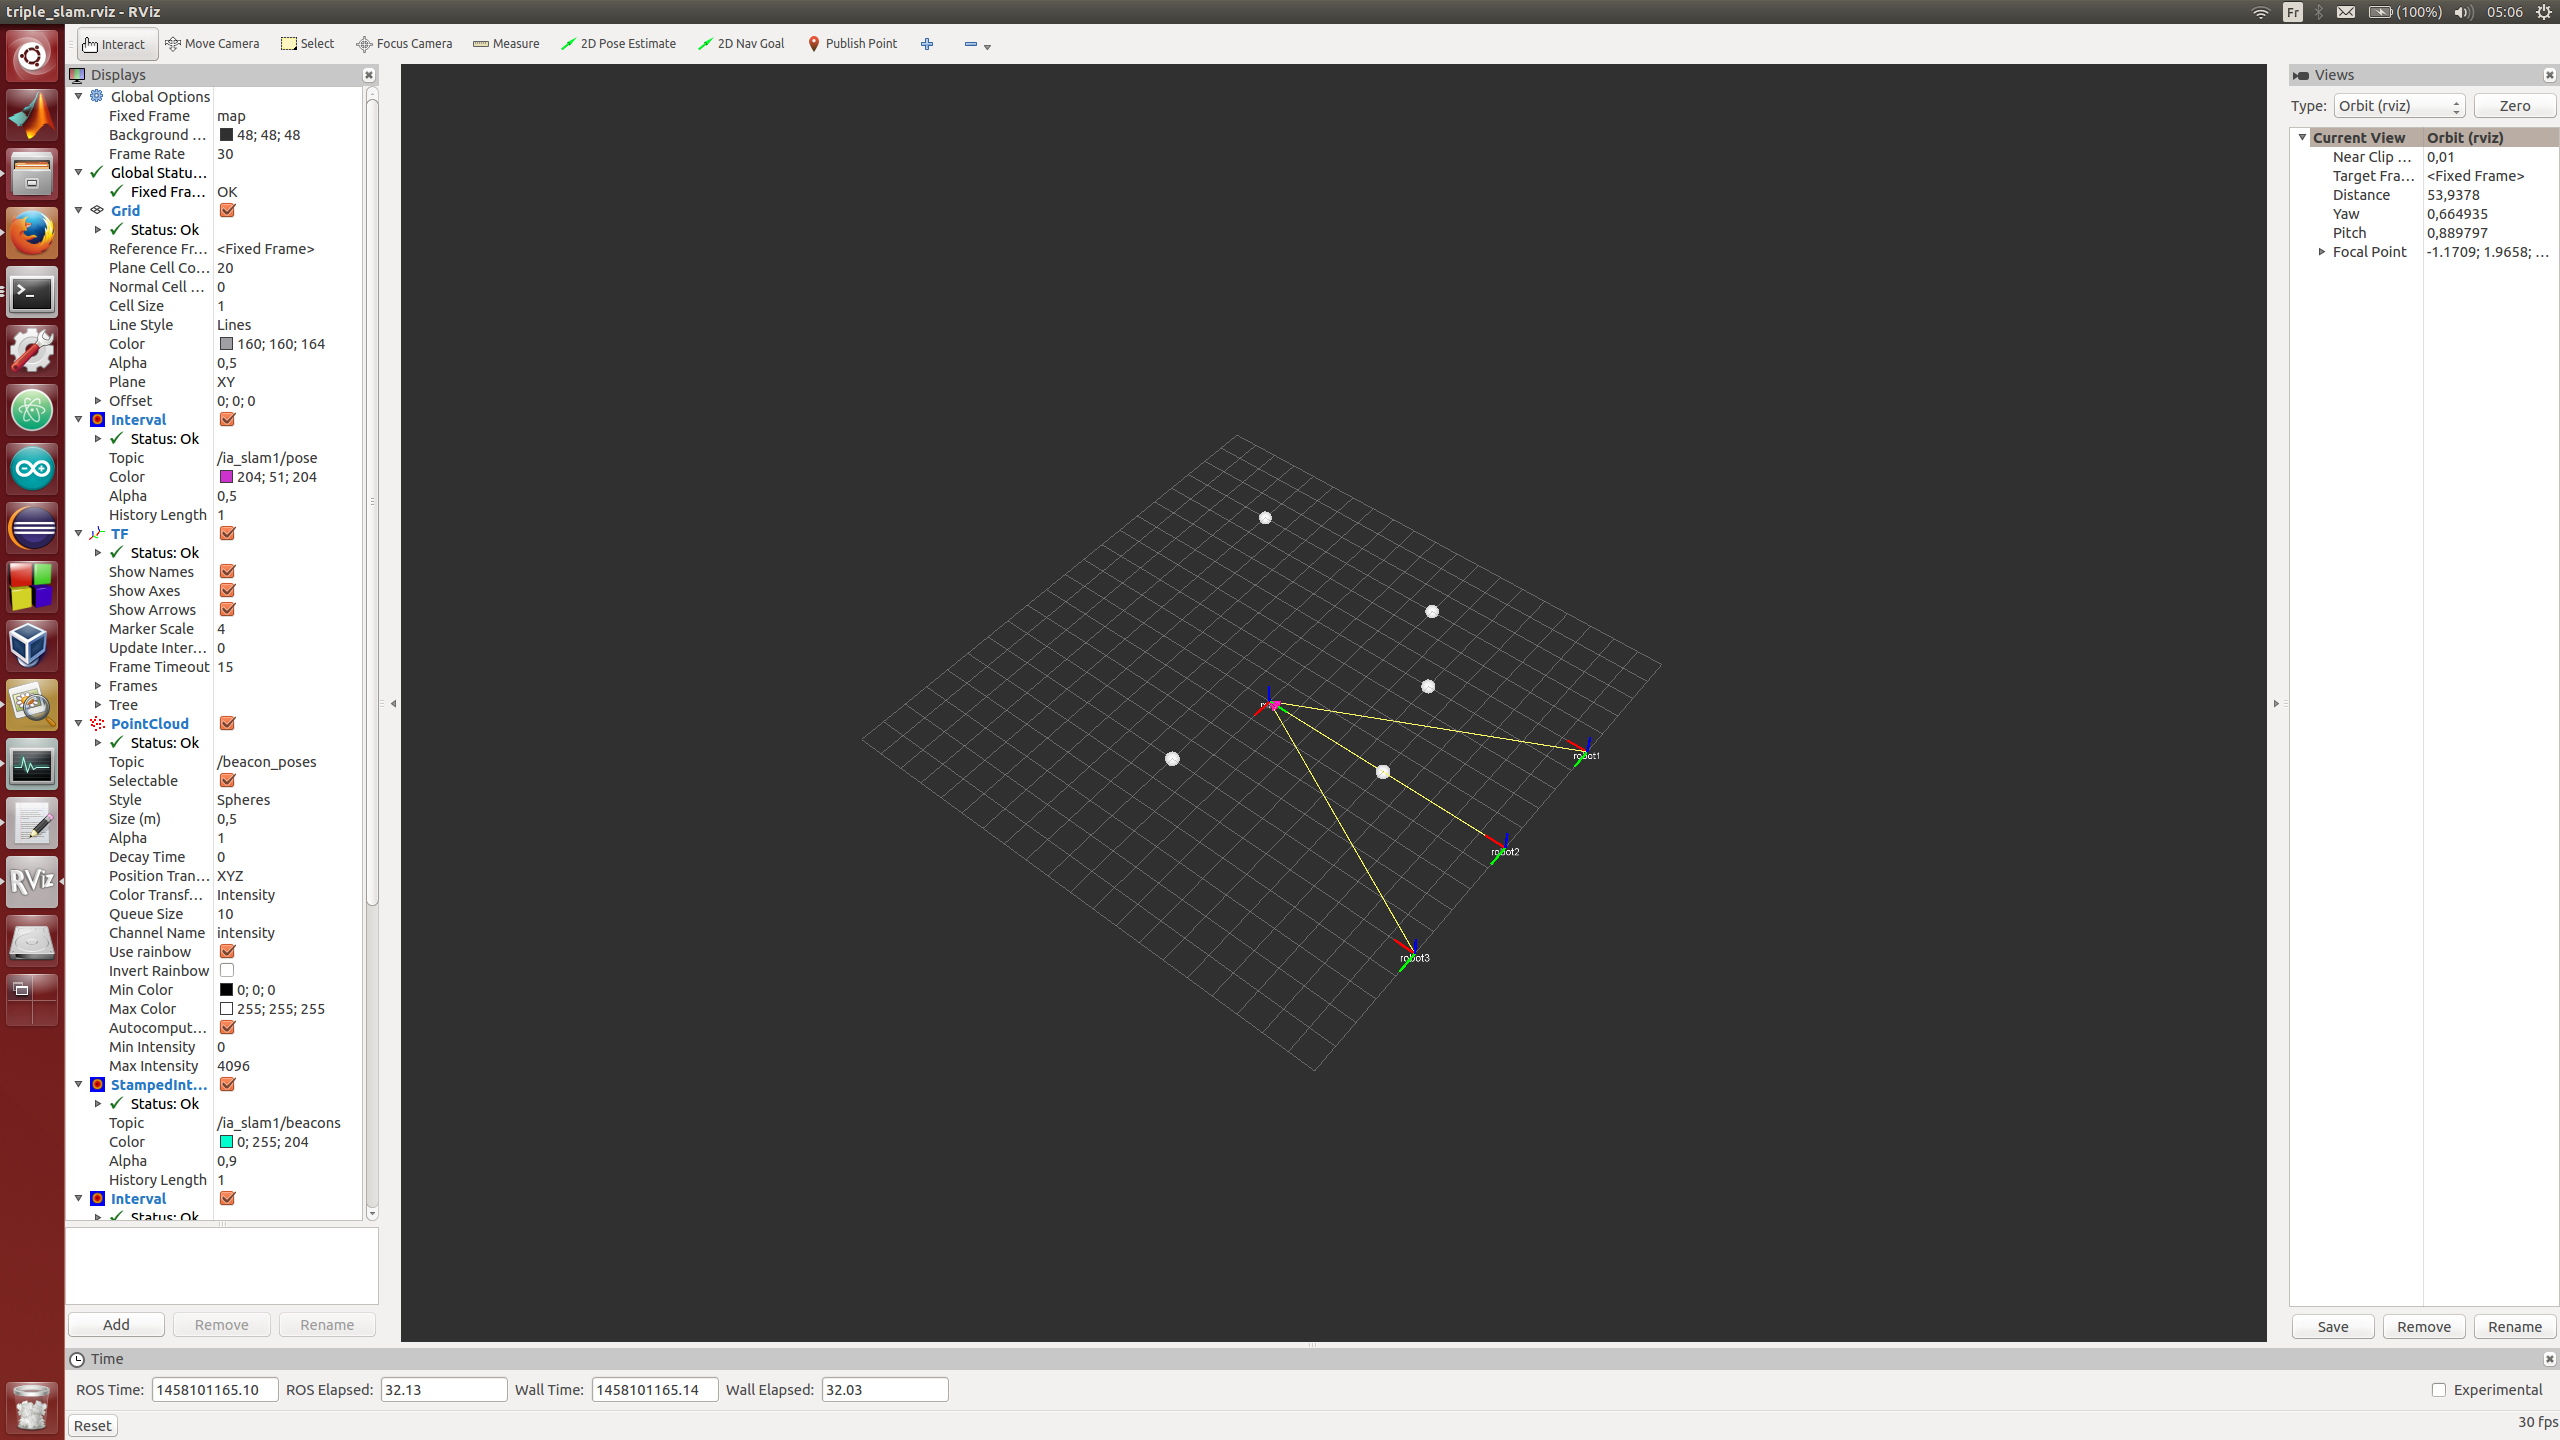
\includegraphics[trim={35cm 15cm 30cm 15cm},clip,scale=0.2,angle=0]{pose_initial.png}
\caption{Initial Poses of the robots.}
\label{fig:initialPose}
\end{figure}

\section{One Robot}

For the test, one robot is used with a sensor precision of 10cm  and a precision for the starting position of 10cm. A case is 1mx1m.

\begin{figure}[H]
\centering
\begin{minipage}[b]{0.4\textwidth}
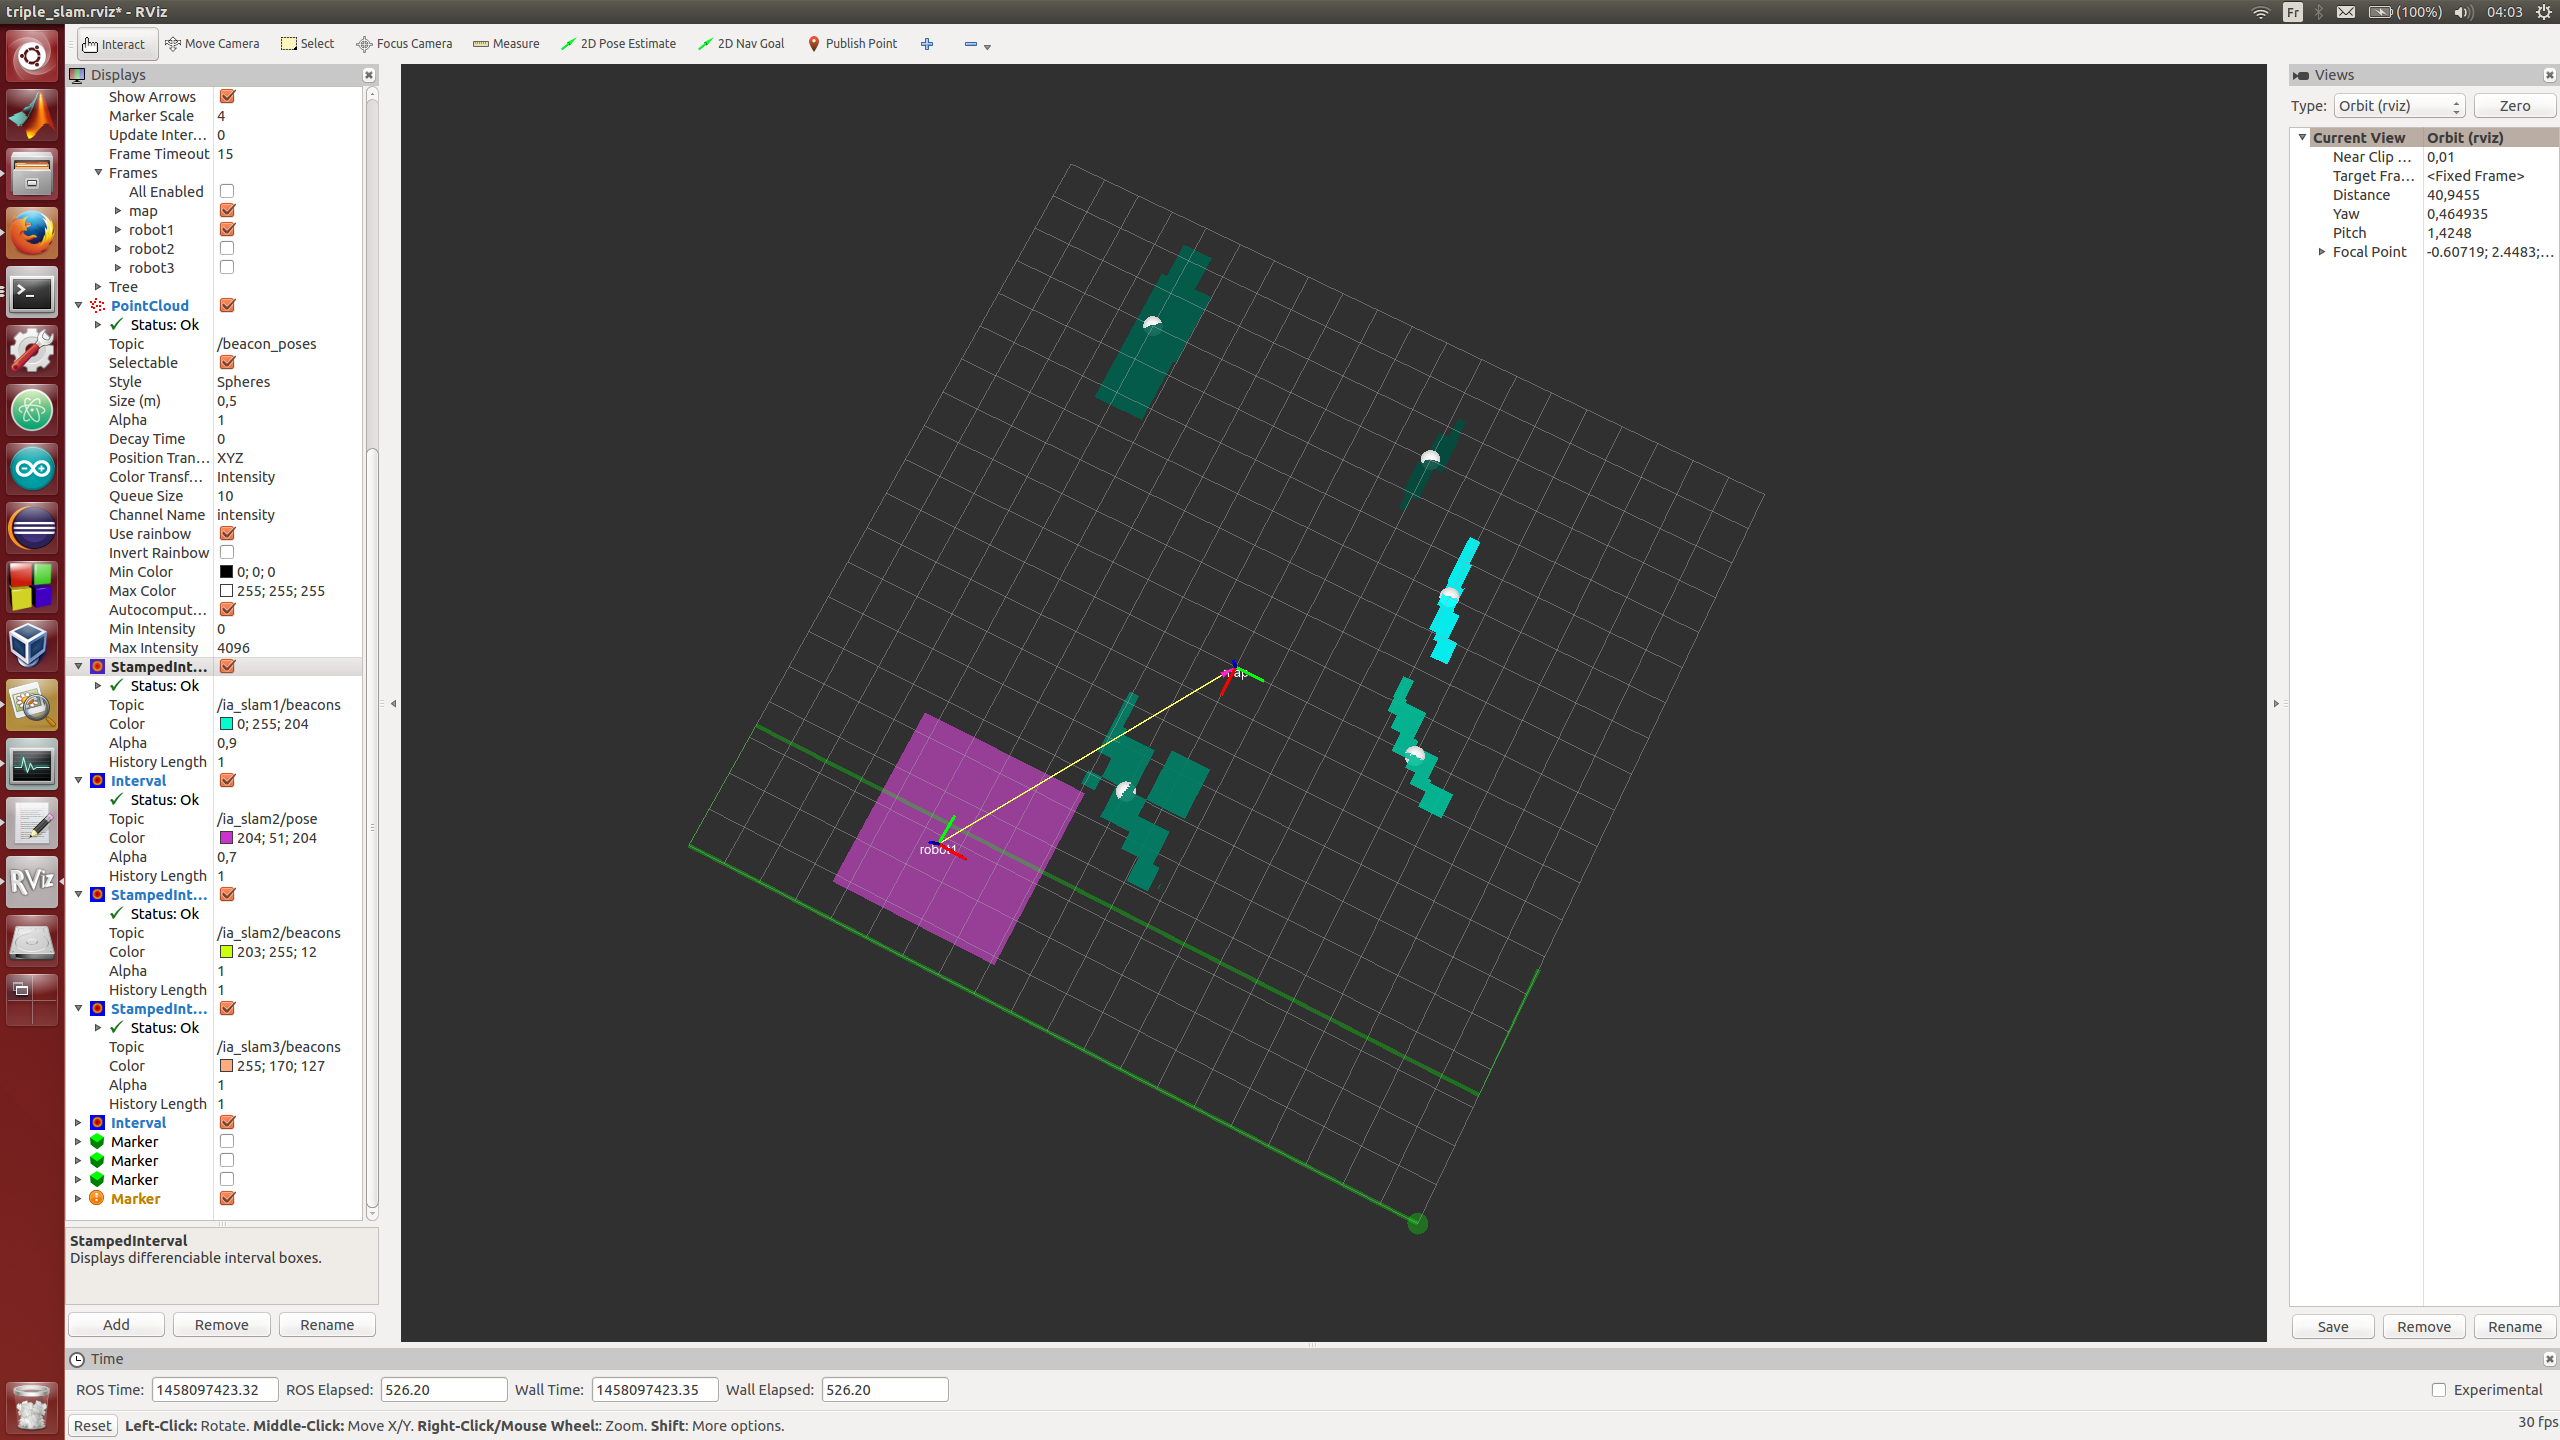
\includegraphics[trim={25cm 7cm 30cm 6cm},clip,scale=0.15,angle=0]{one_robot_result.png}
\caption{Visualization with one robot scanning the area (start).}
\label{fig:oneRobResDeb}
\end{minipage}
\begin{minipage}[b]{0.4\textwidth}
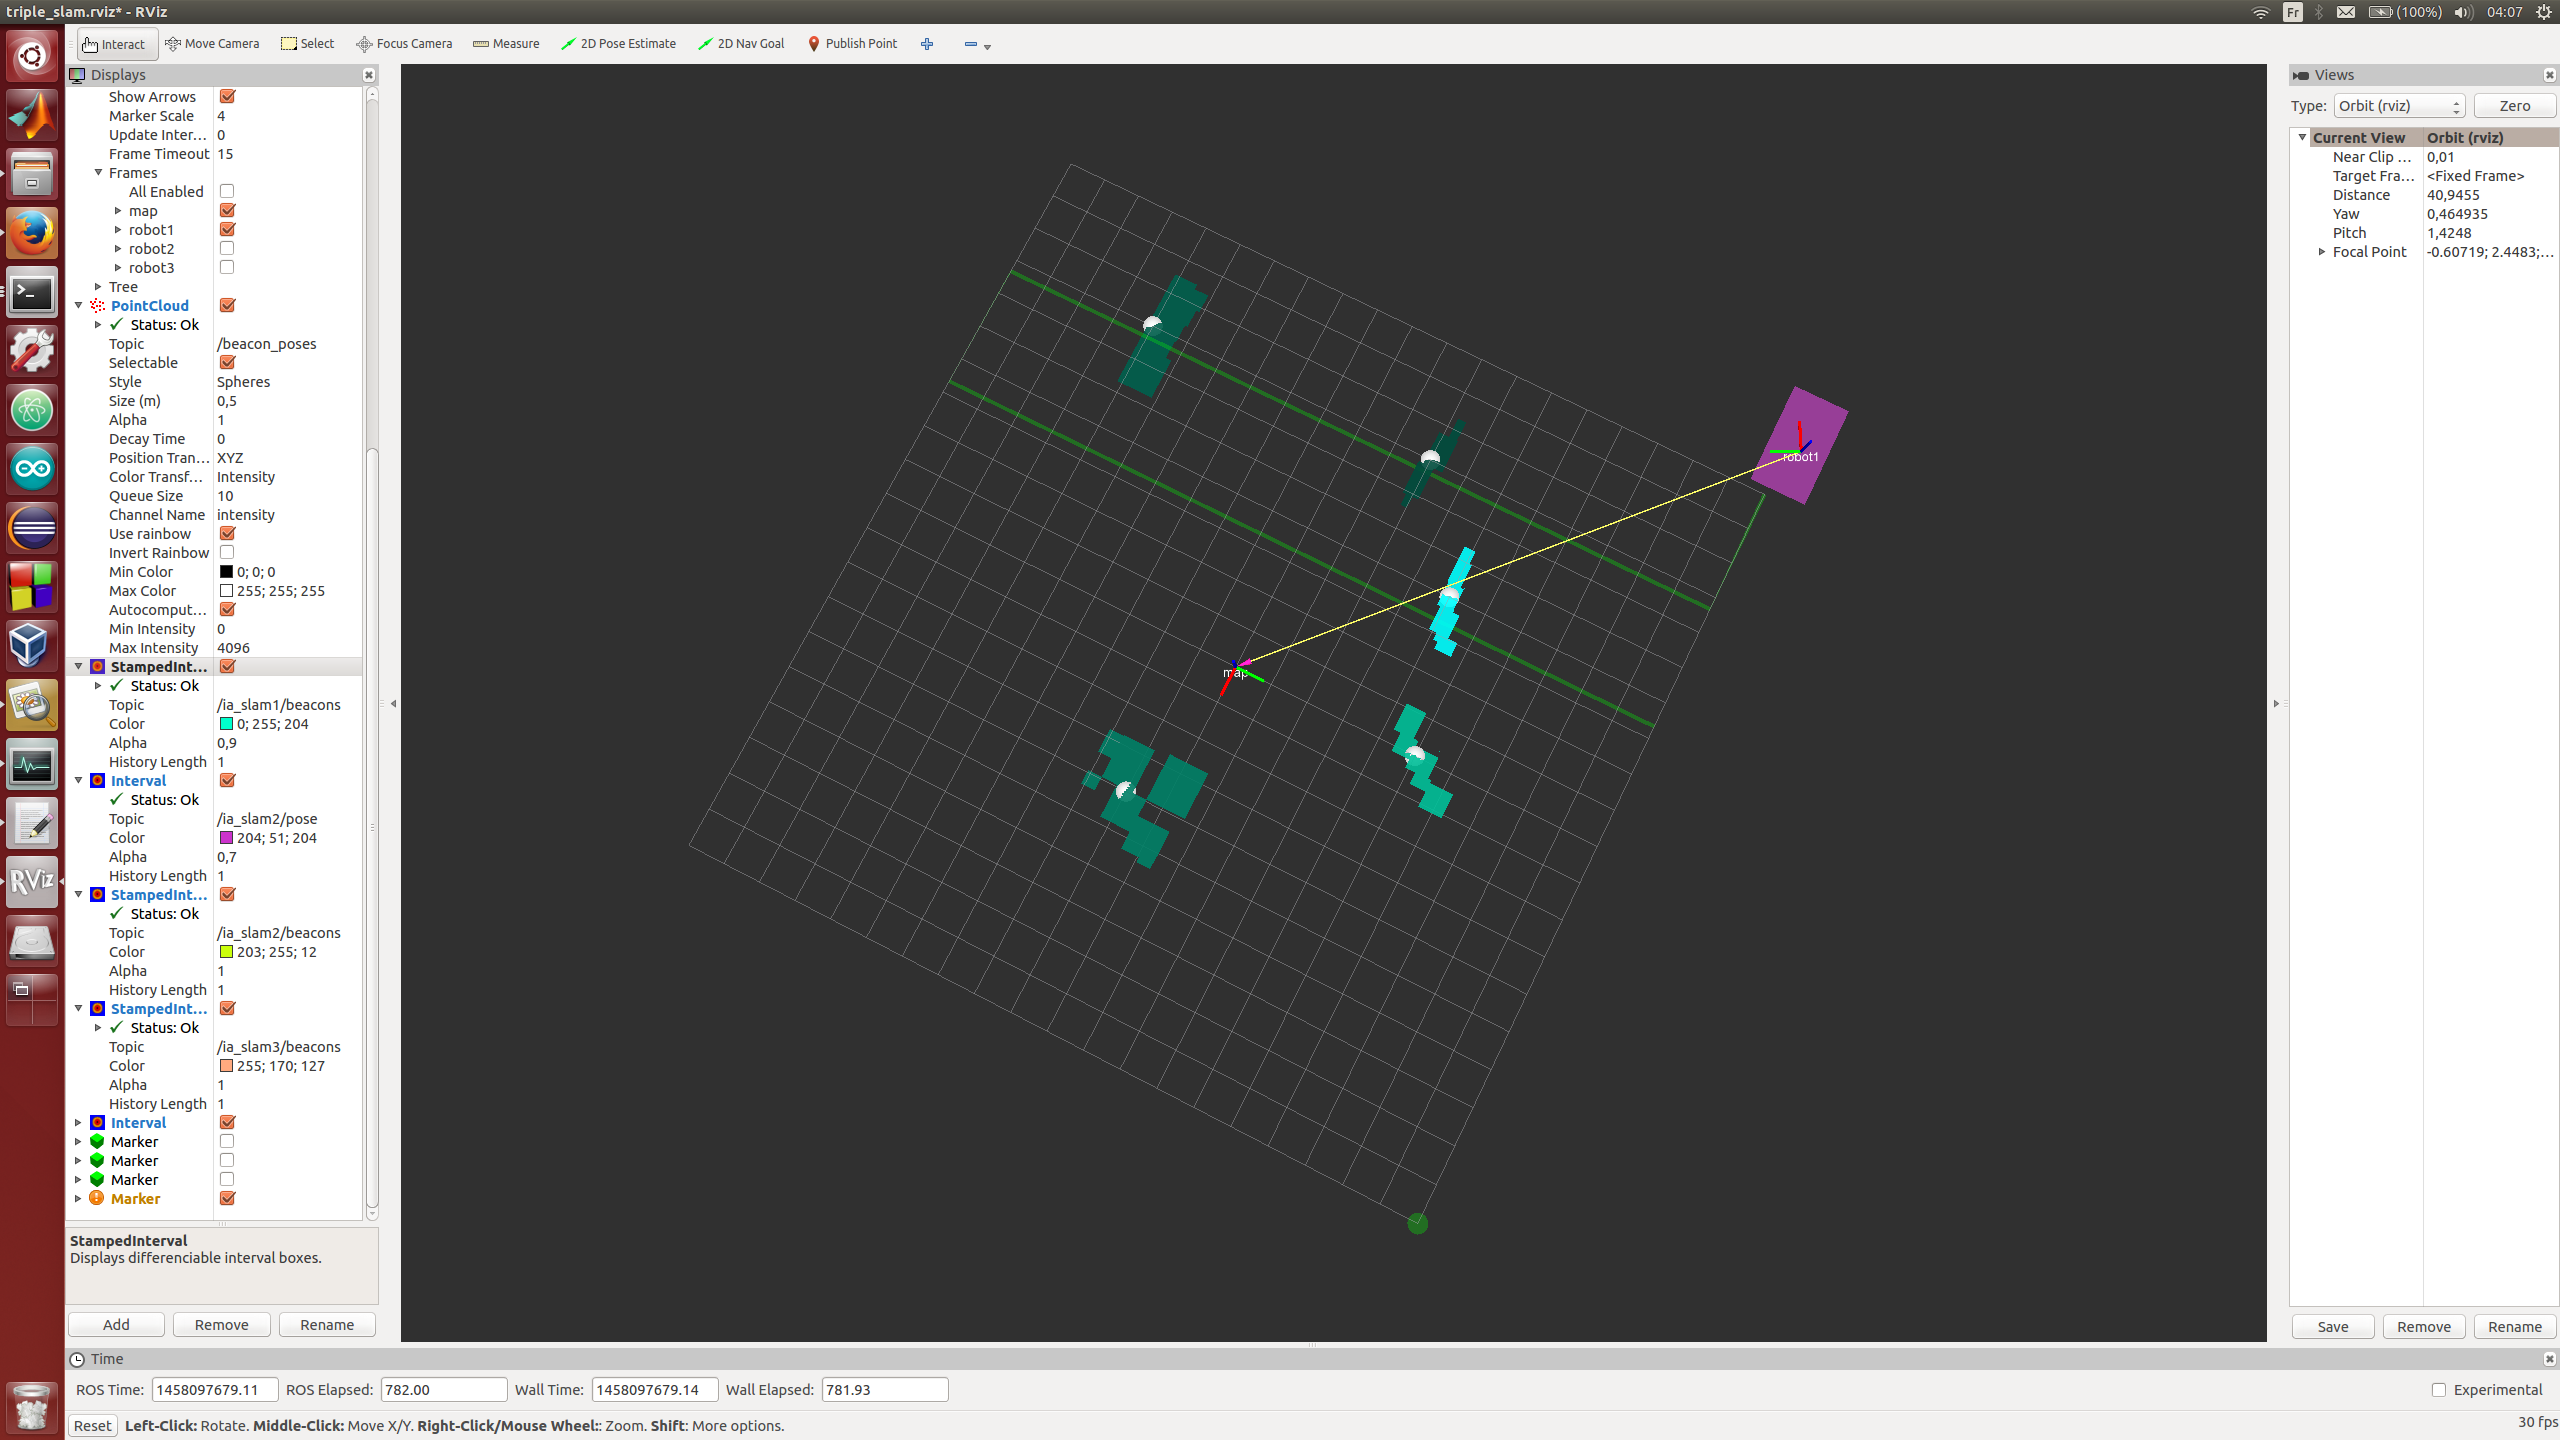
\includegraphics[trim={25cm 7cm 25cm 6cm},clip,scale=0.15,angle=0]{one_robot_result_end.png}
\caption{Visualization with one robot scanning the area (end).}
\label{fig:oneRobResEnd}
\end{minipage}
\end{figure}

The images~\ref{fig:oneRobResDeb} and~\ref{fig:oneRobResEnd} are obtained with the robot going directly to the scanning without doing the first pass (see subsection~\ref{ssec:pathgen}).

The estimate of the beacons has not got good quality the estimate for one beacon are spread out around it therefore the estimate of the robot  is not good and consequently the controller can't correctly handle the robot and in figure~\ref{fig:oneRobResDeb} the robot does not follow exactly the path (green line) and has an offset.

\section{Two Robots}

For this test, one robot is used with a sensor precision of 10cm  and a precision for the starting position of 70cm. In this test the second robot follows the same path as the first one.

\begin{figure}[H]
\centering
\begin{minipage}[b]{0.4\textwidth}
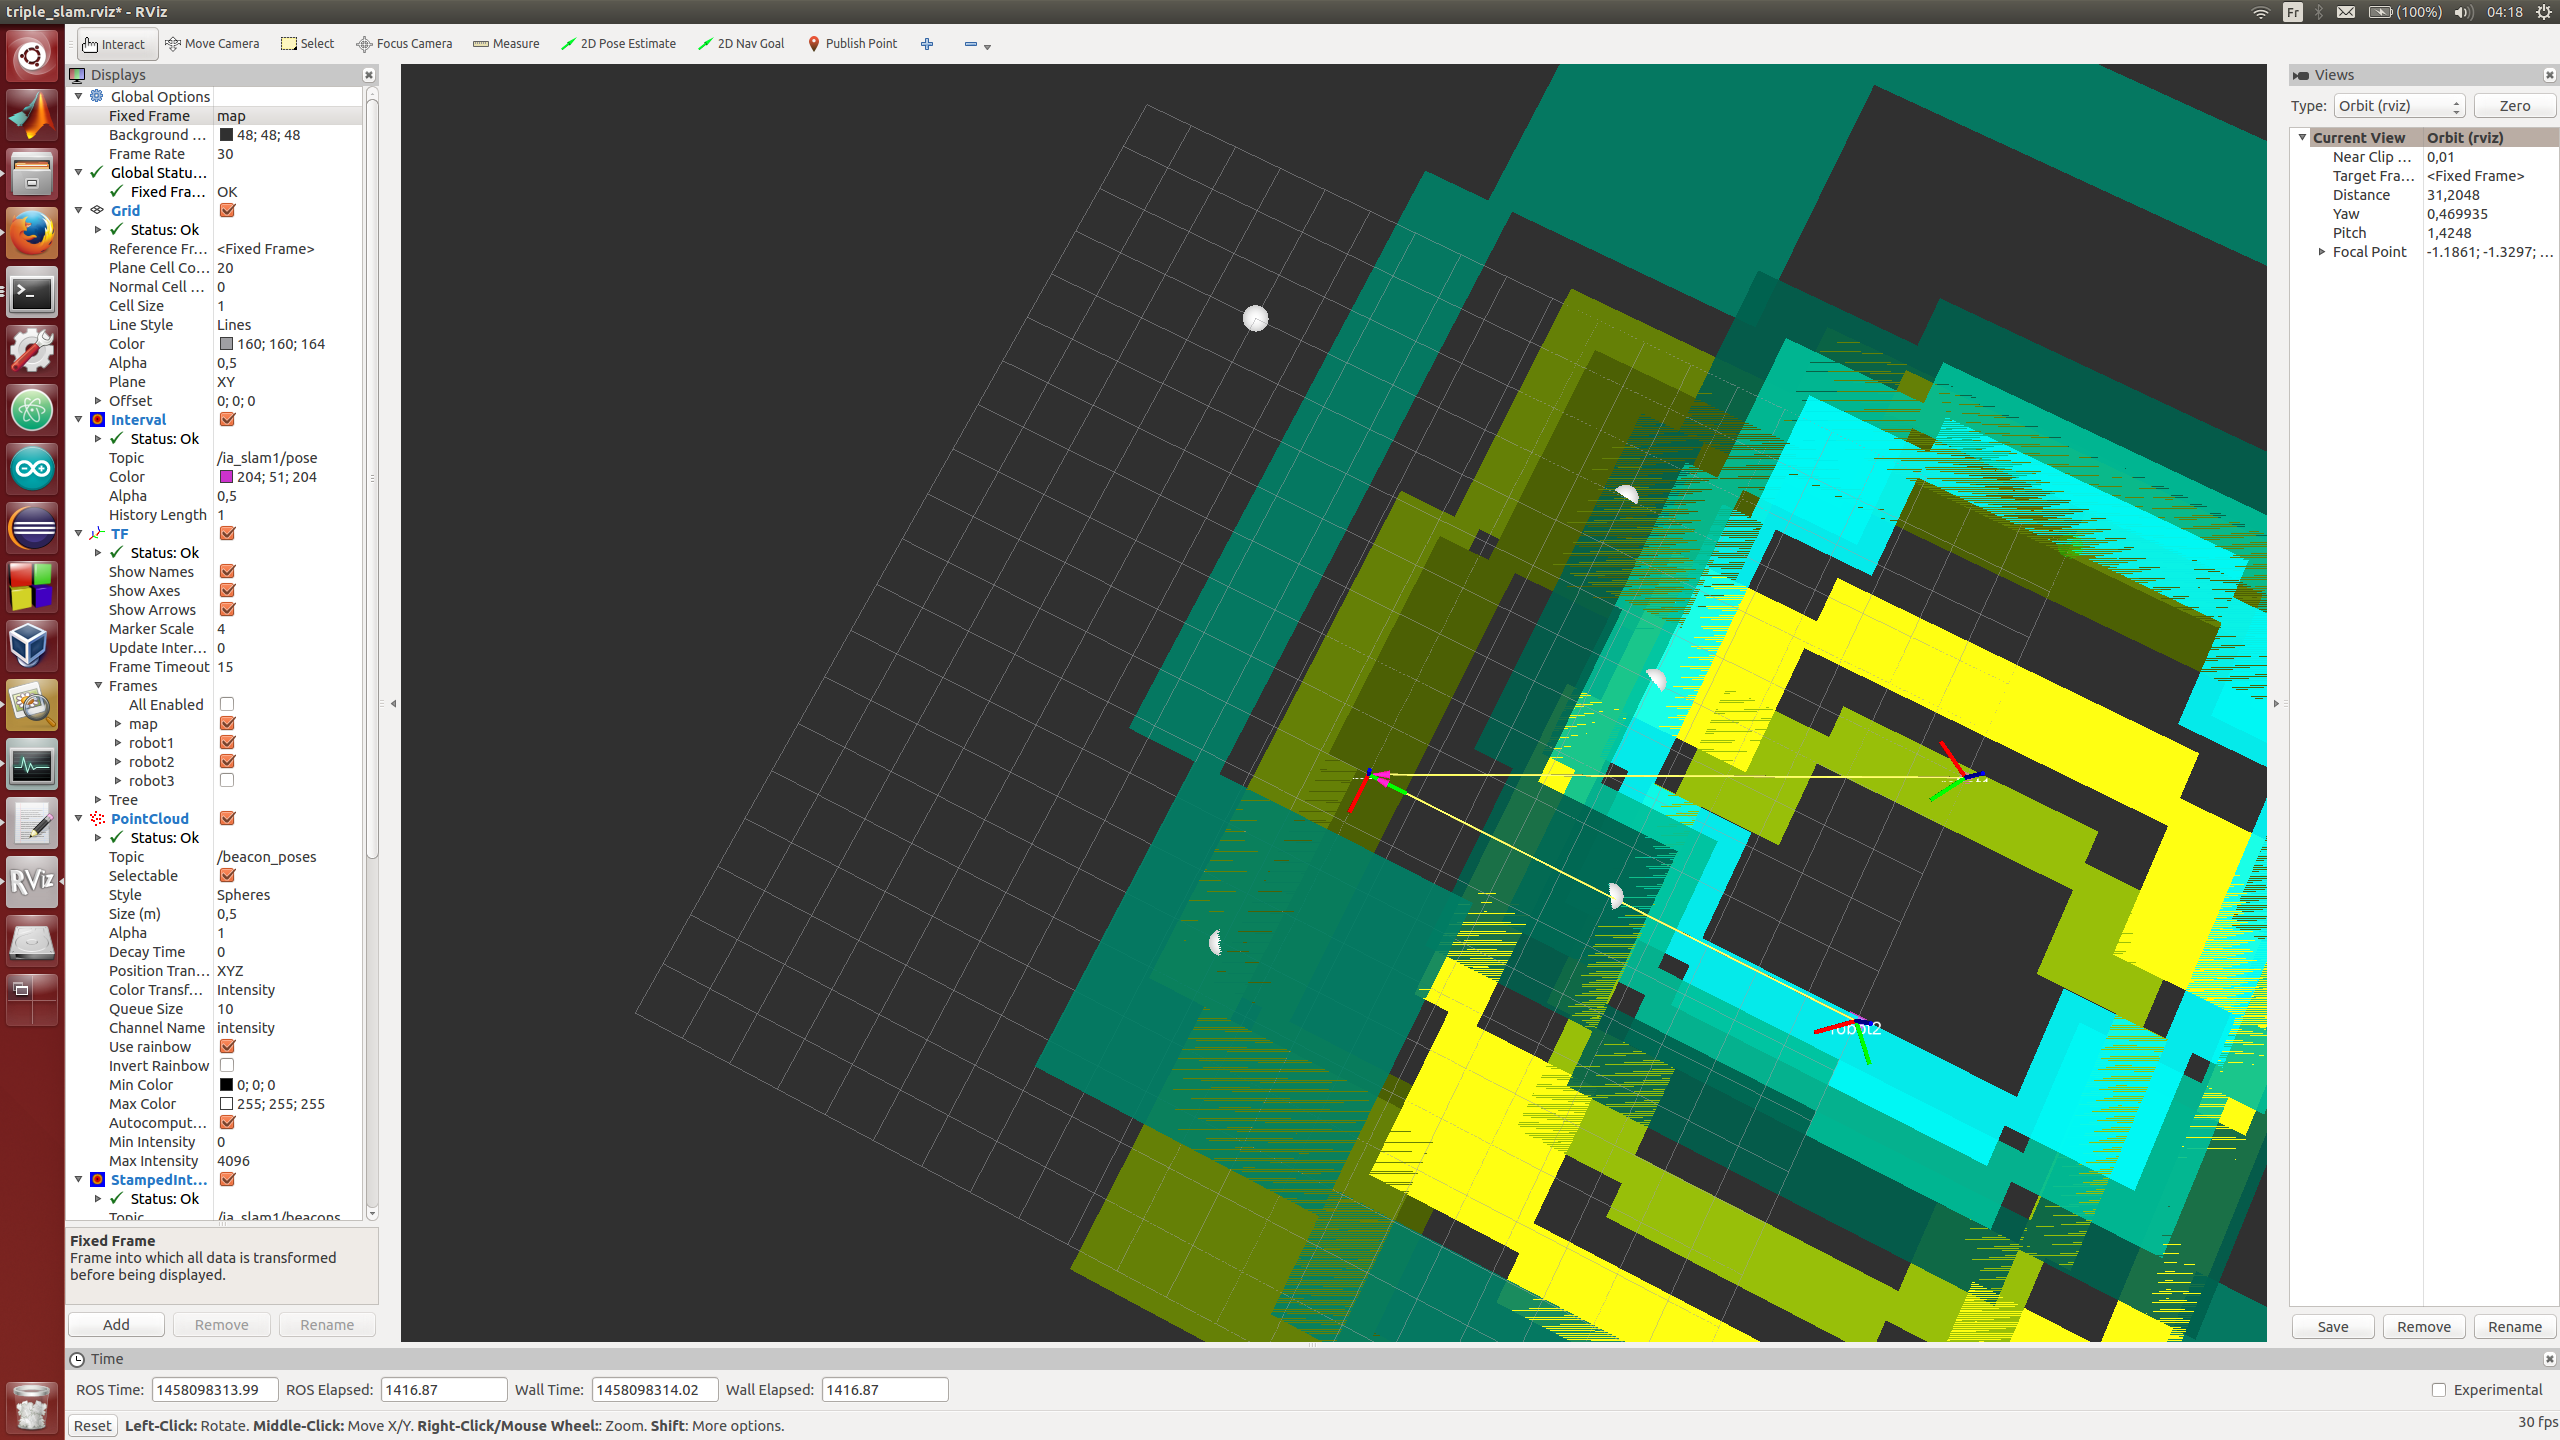
\includegraphics[trim={33cm 7cm 20cm 6cm},clip,scale=0.15,angle=0]{start_two.png}
\caption{Visualization of start of the slam without discussion between robots.}
\label{fig:twoRobResDeb}
\end{minipage}
\begin{minipage}[b]{0.4\textwidth}
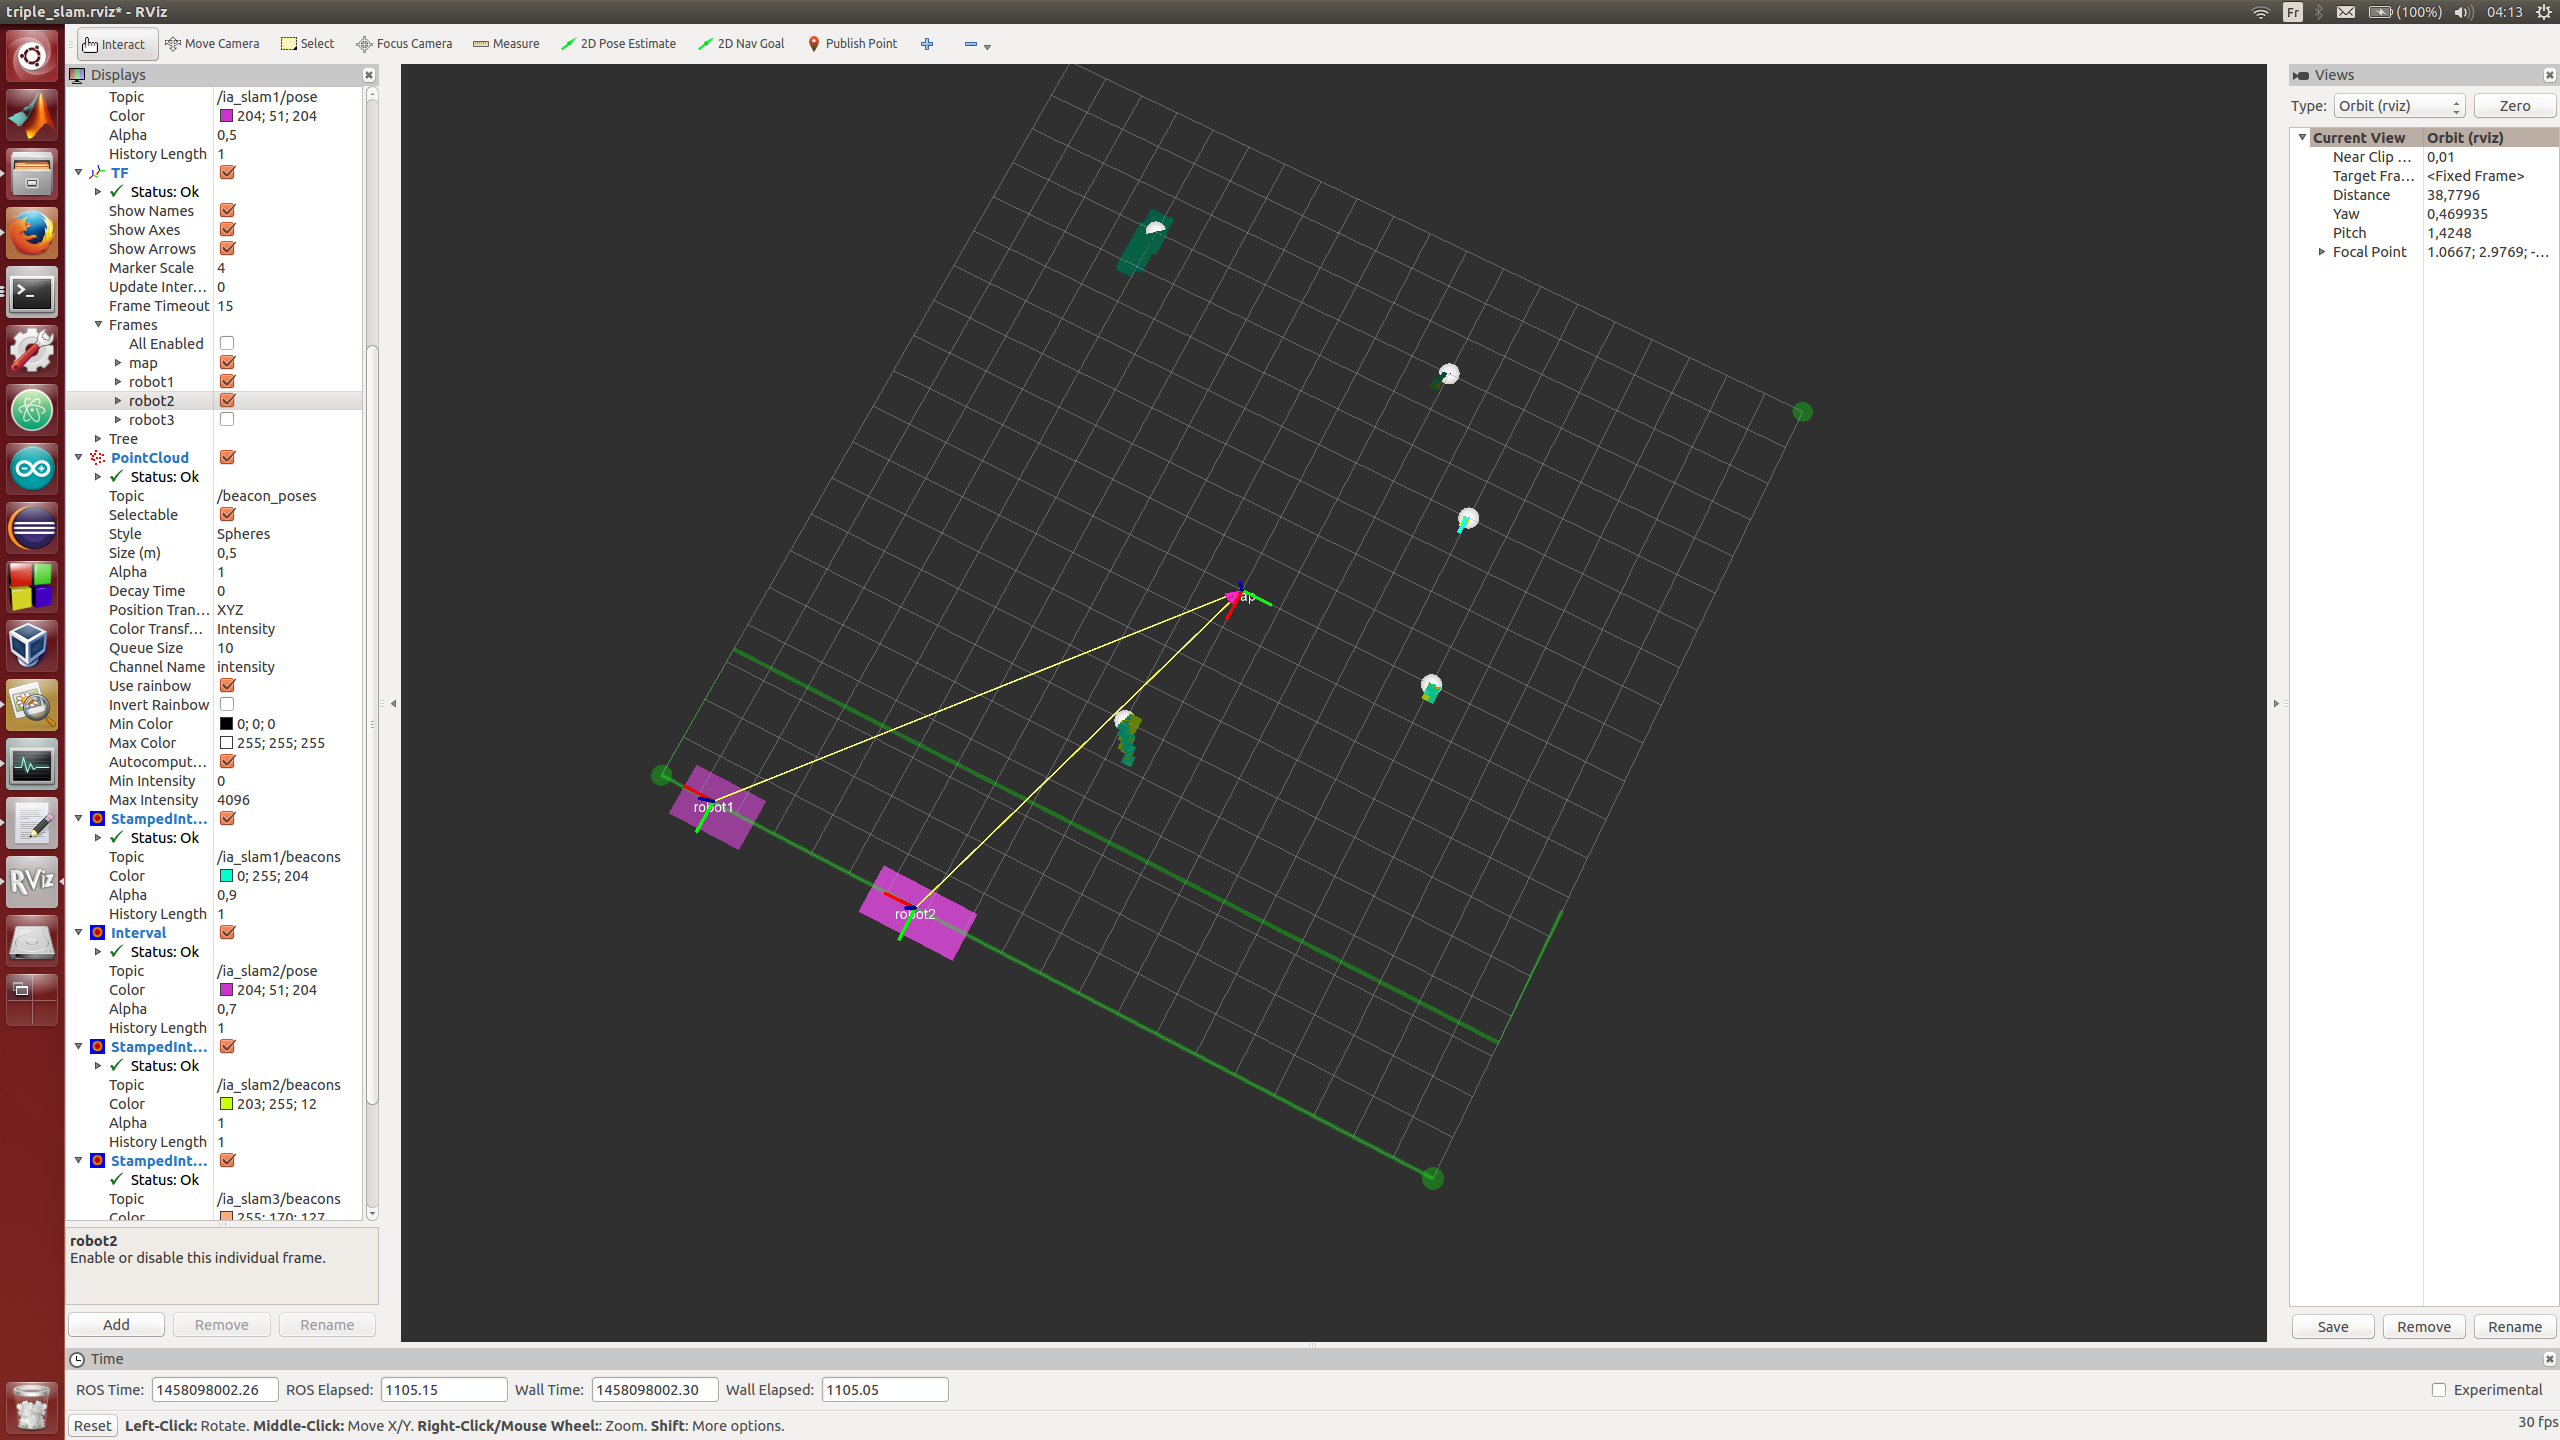
\includegraphics[trim={20cm 7cm 30cm 6cm},clip,scale=0.15,angle=0]{two_robot_start_scanning.png}
\caption{Visualization of the two robots following the scanning path.}
\label{fig:twoRobResEnd}
\end{minipage}
\end{figure}

With two robots communicating the estimations become more precise and allow a better path following(figure~\ref{fig:twoRobResEnd}.
From them the it could continue to more robots but some errors have happened. Indeed sometime the estimation for a beacon is wrong, the boxes do not include the beacon. 

\begin{figure}[H]
\centering
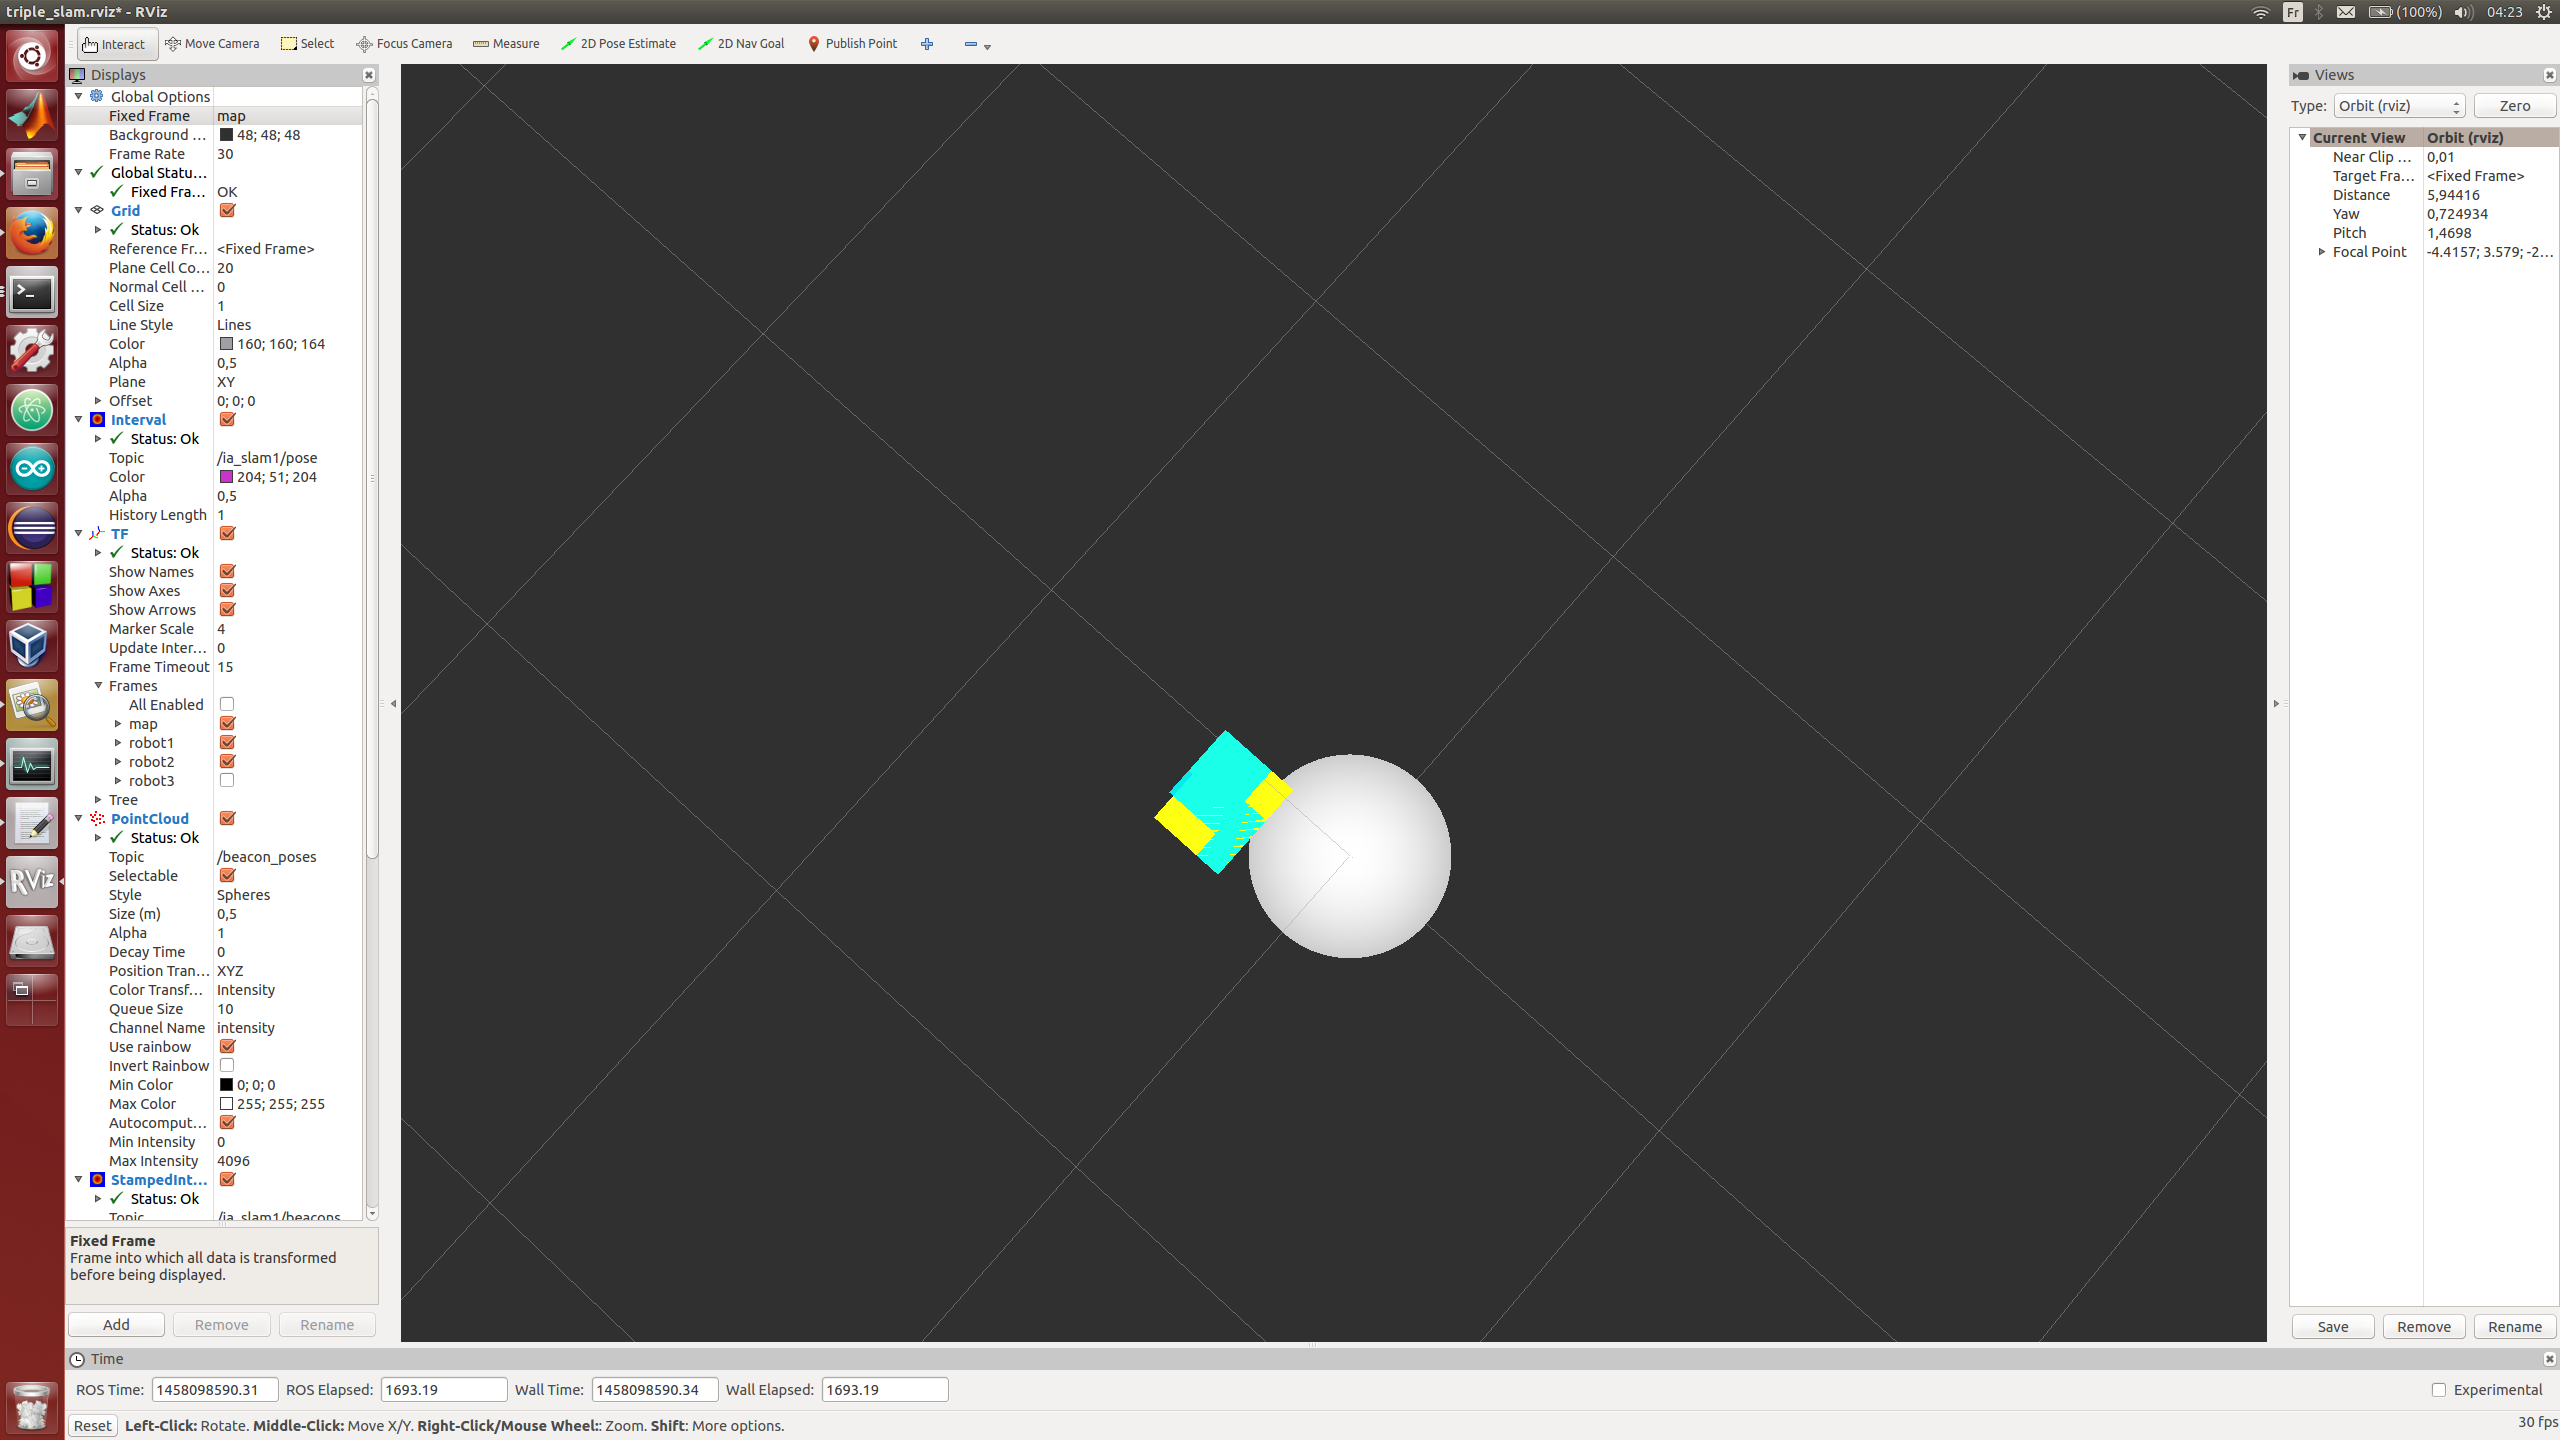
\includegraphics[trim={35cm 15cm 30cm 15cm},clip,scale=0.2,angle=0]{error.png}
\caption{Error on the beacon estimate.}
\label{fig:errorEst}
\end{figure}

The interval method is supposed to give a guaranteed results therefore the problem has to come from the implementation,either there is wrong data in the input,dela in communication is too important(see subsection~\ref{ssec:delaycompProb}), or the state equation used is wrong( but it is working for the robot alone).
By repeating the test it can be seen that the problem originates from the start of the test and there is wrong calculation on the pose estimate.
\chapter*{Conclusion}
% facilite comment ca c fait a implementer 
%long a fairele slam
%tuner en fonction du pc
%generally pessimiste 

% a faire
%refactoring
%optimization
%correction of errors
%passage trois dimension
%more path possibilite 
%real experiment
\addcontentsline{toc}{part}{Conclusion}
%----------------------------------------------------------------------------------------
%%\appendix
\chapter{Appendix 1}

\begin{figure}[H]
\centering
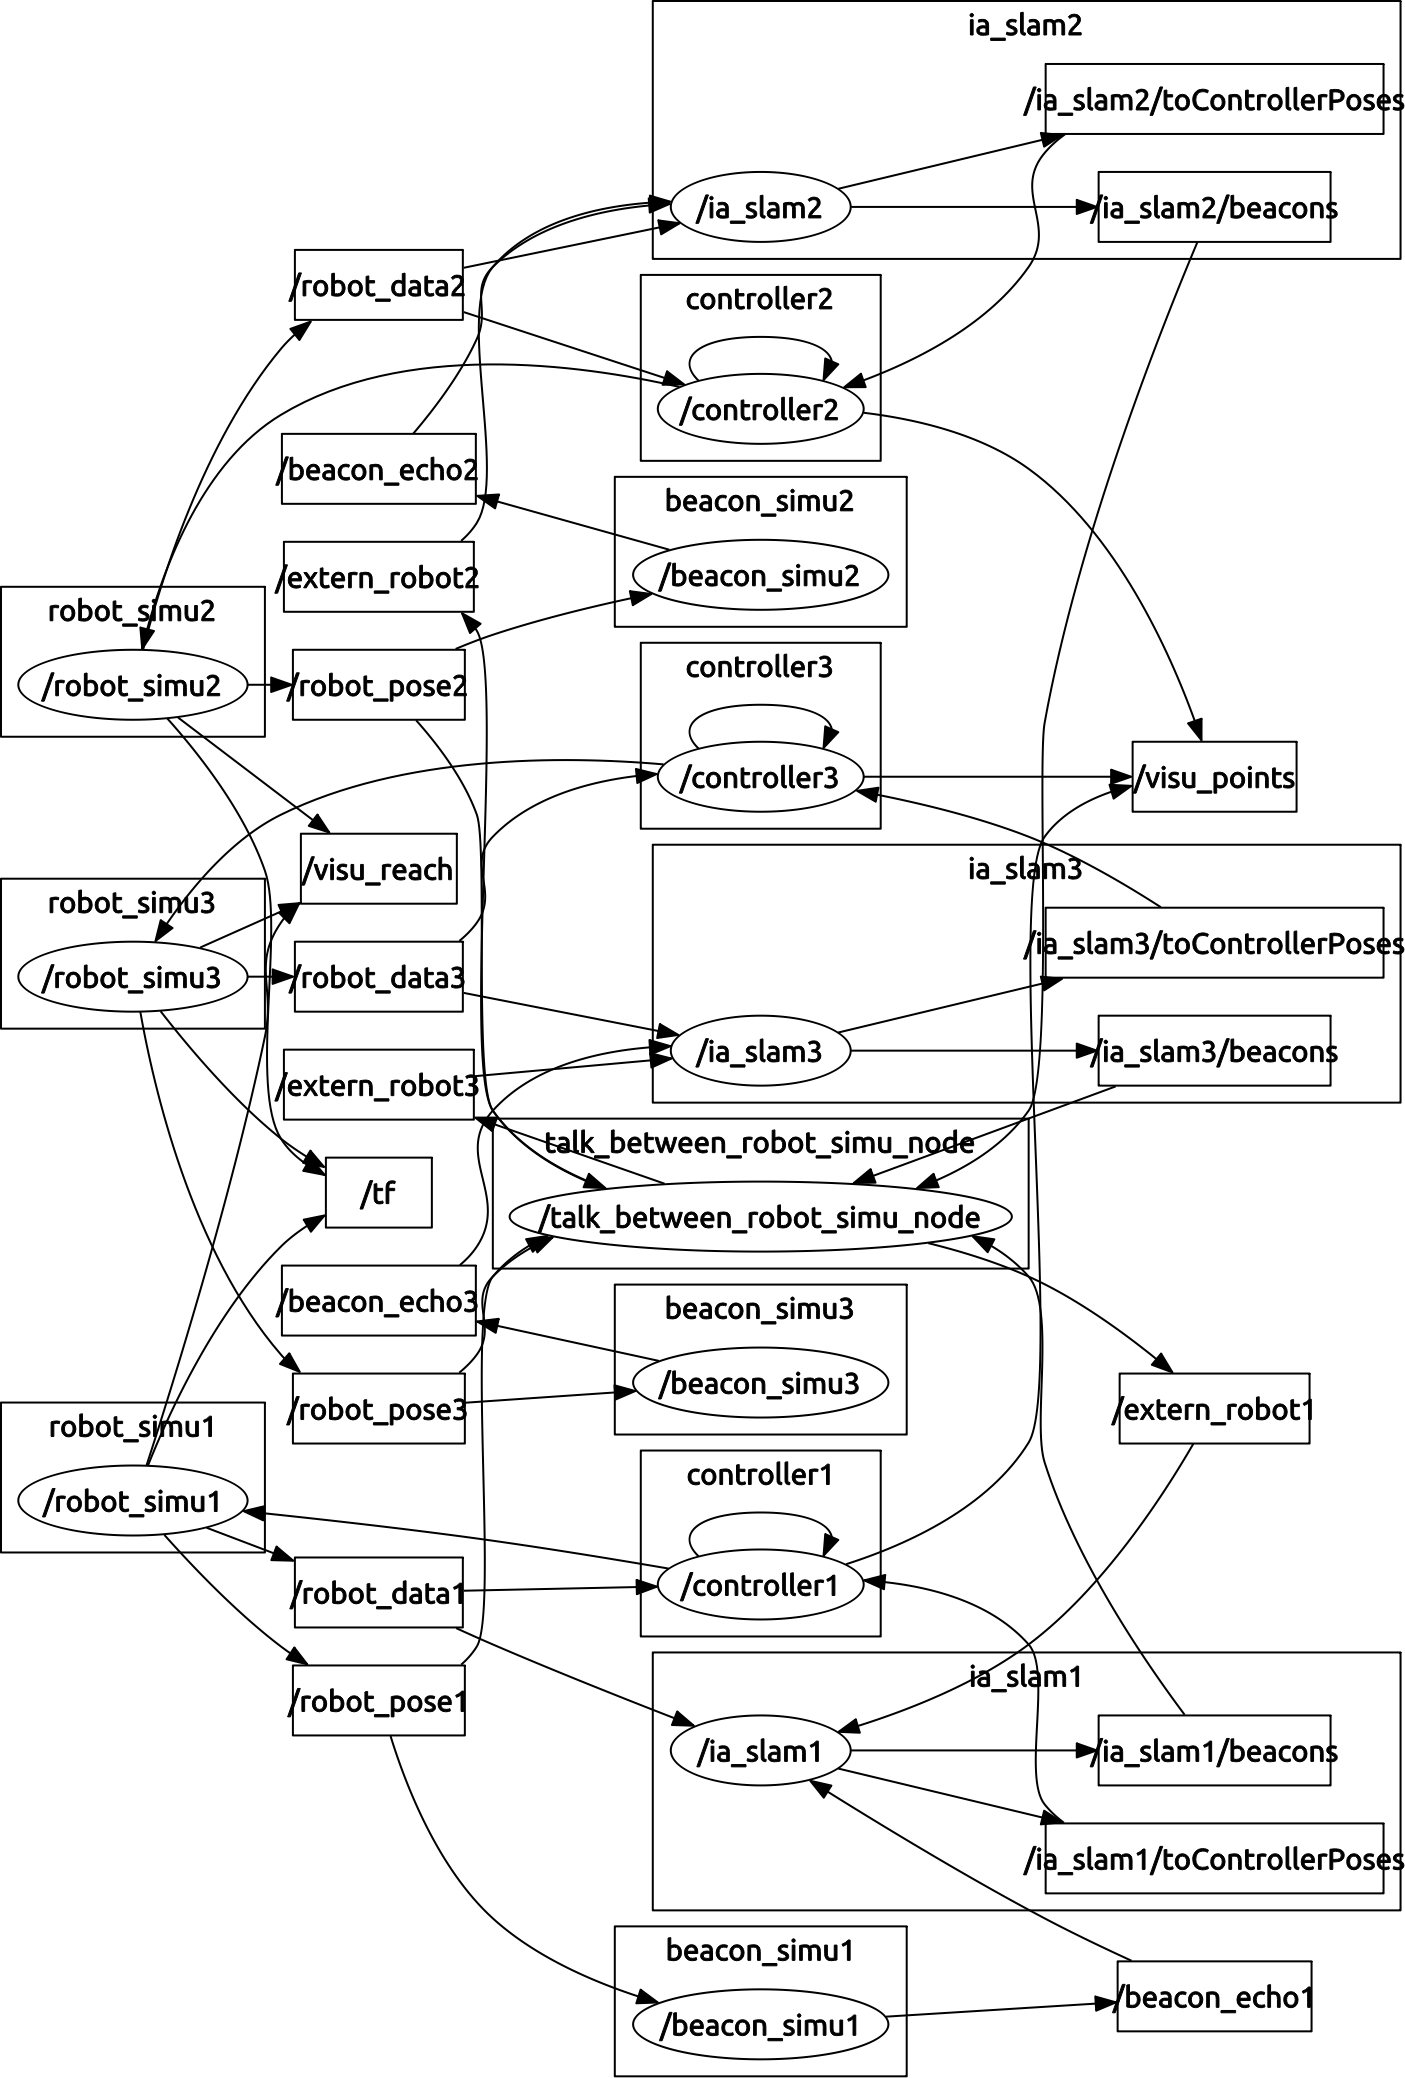
\includegraphics[scale=0.3]{rosgraph.png}
\caption{Relation between node with a simulation of three robots}
\label{fig:completeNode}
\end{figure}


%%\chapter{Appendix 2}
%%\chapter{Appendix 3}
%----------------------------------------------------------------------------------------
%	BIBLIOGRAPHIE
%----------------------------------------------------------------------------------------
%\addcontentsline{toc}{part}{Bibliography}
%\bibliographystyle{apalike-fr}
\bibliographystyle{IEEEtran}
\bibliography{bibliographie}
\addcontentsline{toc}{part}{Bibliography}
\nocite{*}




%----------------------------------------------------------------------------------------

\end{document}